\chapter{Desarrollo. Entregas e iteraciones}
\label{ch:desarrollo}
Este capítulo recoge el proceso de desarrollo del juego, en el que se detallan las diferentes entregas e iteraciones, así como los resultados de estas.

\section{Entrega 0}
En esta entrega se ha llevado a cabo una prueba de viabilidad del proyecto, en la que se ha comprobado como funciona el SDK ARCore, y que posibilidades ofrece. La prueba que se llevó a cabo consistía en asociar diferentes elementos 3D a diferentes imágenes.\\

En la Figura \ref{figura-demo-tablero} se puede observar la demo en funcionamiento, en ella la aplicación reconoce la imagen del tablero de juego y le asocia un cubo 3D que se muestra en el centro del tablero.

\begin{figure}[h]
  \centering
  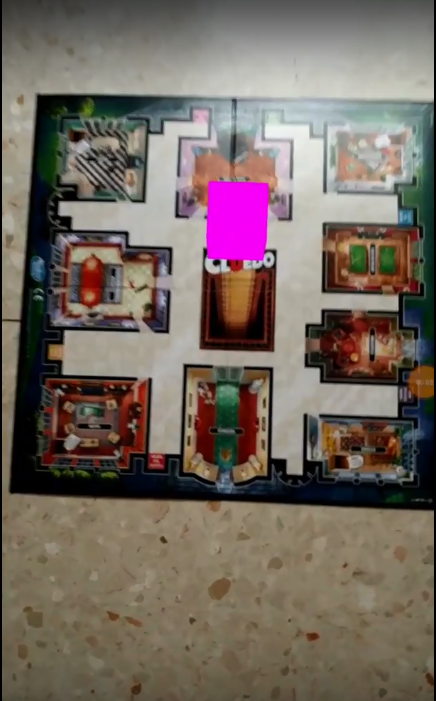
\includegraphics[scale=0.25]{demo-tablero}
  \caption{Imagen que muestra la demo en la que hay un objeto 3D asociado al tablero de juego.}
  \label{figura-demo-tablero}
\end{figure}

\newpage
En la Figura \ref{figura-demo-imagenes} se puede observar la demo en funcionamiento, en ella la aplicación reconoce la imagen del tablero y las de diferentes habitaciones y asocia diferentes elementos 2D a cada una de las imágenes.

\begin{figure}[h]
  \centering
  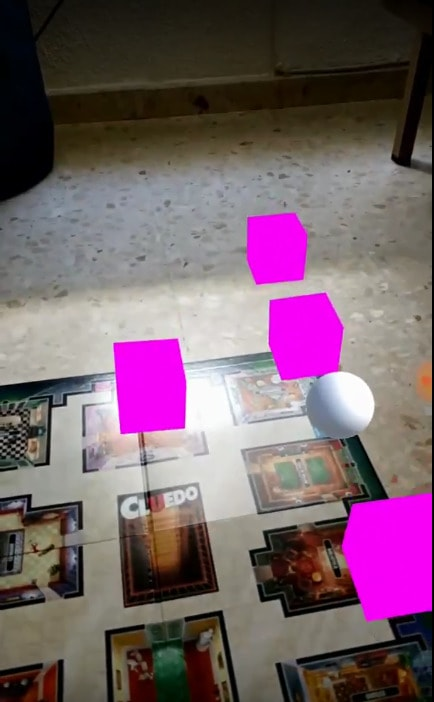
\includegraphics[scale=0.25]{demo-imagenes}
  \caption{Imagen que muestra la demo en la que hay objetos 3D asociados al tablero y diferentes habitaciones.}
  \label{figura-demo-imagenes}
\end{figure}

A continuación se muestra en la Figura \ref{figura-codigo} un extracto de código de ARCore.

\begin{figure}[h]
  \centering
  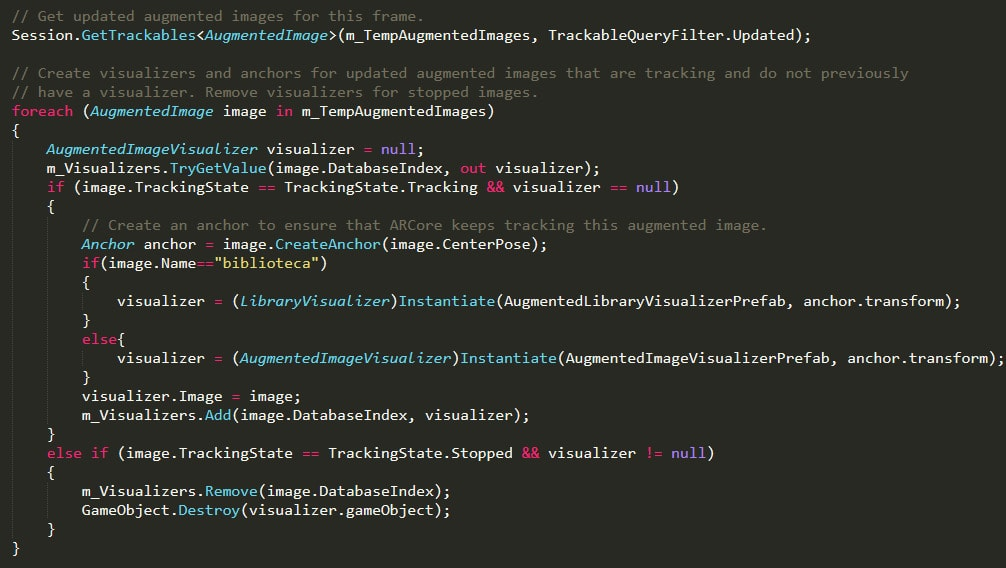
\includegraphics[width=15cm,height=9cm]{codigo-arcore}
  \caption{Imagen que muestra código de ARCore.}
  \label{figura-codigo}
\end{figure}

\FloatBarrier

En este encontramos diferentes elementos relevantes:

\begin{itemize}
  \item \textbf{Session.GetTrackables<AugmentedImage>(mTempAugmentedImages, TrackableQueryFilter.Updated)}: Este código hace una llamada para obtener las imágenes aumentadas que han sido localizadas en la imagen percibida por la pantalla.

  \item \textbf{if (image.TrackingState == TrackingState.Tracking && visualizer == null)}: Este código comprueba que se conozca la posición de la imagen en el mundo físico y en caso de así ser y no haber situado un modelo 3D, se entra en el if.

  \item \textbf{Anchor anchor = image.CreateAnchor(image.CenterPose)}: Se crea un ancla en el mundo real con la posición de la imagen, para que así la información asociada a dicha imagen se sitúe en el lugar adecuado.

  \item \textbf{if(image.Name=="biblioteca")}: En caso de que la imagen escaneada sea una biblioteca entra en dicho if donde asignará un objeto de diferente tipo que en el else al visualizador (visualizer). Esto se hace de esta manera ya que si la imagen es de la habitación biblioteca tendrá que colocar un objeto diferente que en el resto de habitaciones, esto se puede comprobar en la Figura \ref{figura-demo-imagenes}.

\end{itemize}

\subsection{Primera iteración}
En esta iteración se ha realizado la demo que se ha mostrado en la \textbf{Entrega 0}.\\

Por otro lado, se ha llevado a cabo una versión inicial del documento de diseño de videojuegos (GDD), que se encuentra en el Apéndice \ref{documento-diseño-videojuegos}, dejando definidos los conceptos iniciales.\\

También se han llevado a cabo las historias de usuario que definen las situaciones en las que un usuario se encontrará cuando quiera llevar a cabo una acción en el juego, estas historias se pueden encontrar en el Apéndice \ref{historias-usuario}, y la lista con las historias de usuario se puede encontrar en el Capítulo \ref{ch:plan}, en la sección "Historias de usuario".\\

Por último en esta iteración se llevó la recopilación de elementos 3D que se utilizarían en el juego.

\subsection{Conclusiones}
Al realizarse la prueba de viabilidad asociando figuras 3D con realidad aumentada a imágenes escaneadas, se pudo comprobar que la realidad aumentada es muy interesante para aplicar en juegos de mesa por las posibilidades que ofrece, permitiendo un realismo que solo un juego de mesa real físico puede alcanzar. Por otro lado se vio que era posible utilizar ARCore para desarrollar un juego junto con el motor Unity, y obtener un resultado satisfactorio.\\

Por otro lado se comprobó que ARCore aun no permite el seguimiento de imágenes en movimiento, por lo que si se mueve el tablero hasta que no lo vuelva a detectar parado no cambia los modelos 3D a esa nueva posición, pero esta característica no era necesaria para nuestro proyecto, ya que al ser un juego de mesa no habrá mucho movimiento.

\section{Entrega 1}
En esta entrega se han llevado a cabo el diagrama de clases del juego que se encuentra en el Apéndice \ref{apendice-diagrama-de-clases}, los bocetos del juego, y pruebas heurísticas y de usuario sobre estos.

%%%%%%%%%%%%%%%%%%%%%%%%%%%%%%%%%%%%%%%%%%%%%%%%%% BOCETOS %%%%%%%%%%%%%%%%%%%%%%%%%%%%%%%%%%%%%%%%%%%%%%%%%%%%%%
\subsection{Bocetos}
Se han creado bocetos que representan la idea inicial del juego y cómo serán sus diferentes pantallas e interfaces, de forma que se puedan utilizar para llevar a cabo pruebas sobre ellos, dichas pruebas incluyen pruebas heurísticas realizadas por el desarrollador y pruebas se usabilidad con usuarios reales, para así saber que esta bien y que no en los bocetos y mejorar el diseño del juego.\\

En la Figura \ref{figura-b1} se puede ver el boceto creado para la pantalla inicial en la que se seleccionará los personajes con los que se quiere jugar:

\begin{figure}[h]
  \centering
  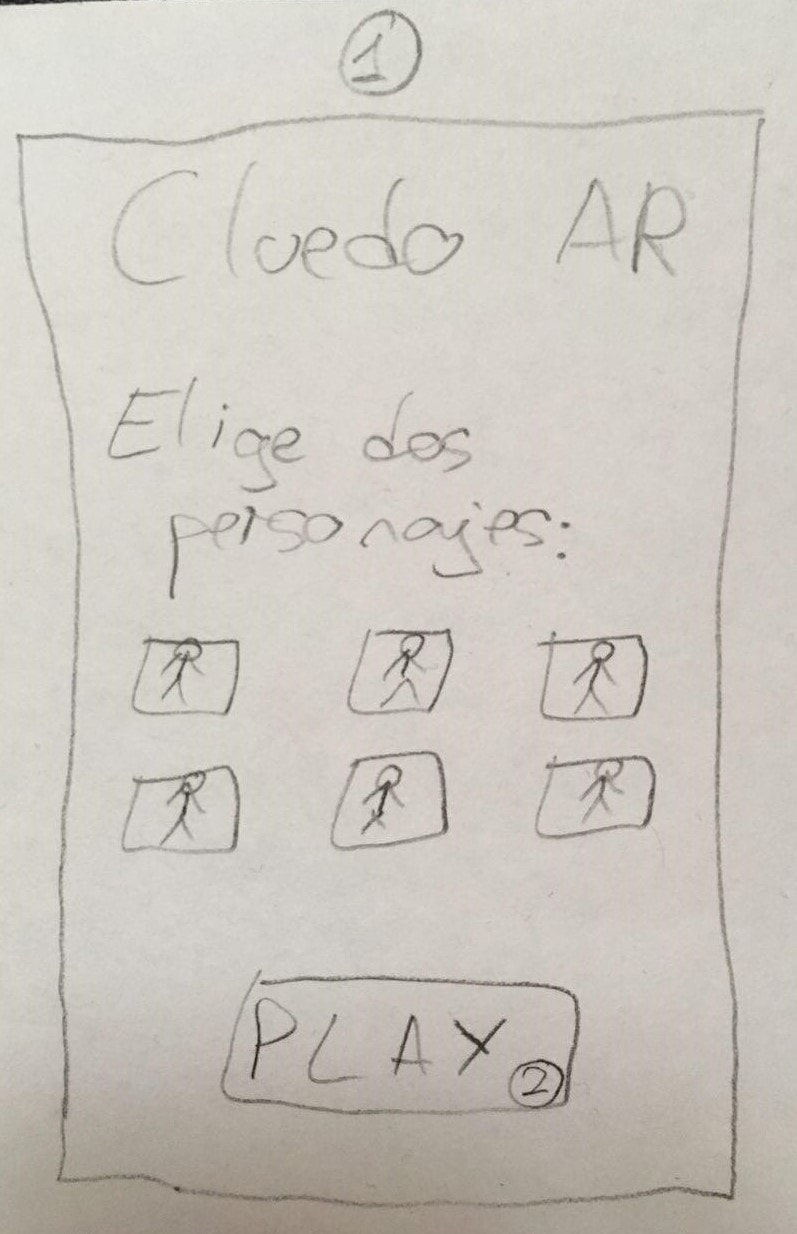
\includegraphics[scale=0.2]{b1}
  \caption{Imagen que muestra la interfaz de la pantalla inicial del juego.\protect\footnotemark}
  \label{figura-b1}
\end{figure}

\newpage

En la Figura \ref{figura-b2} se puede ver el boceto creado para la pantalla de instrucciones:

\begin{figure}[h]
  \centering
  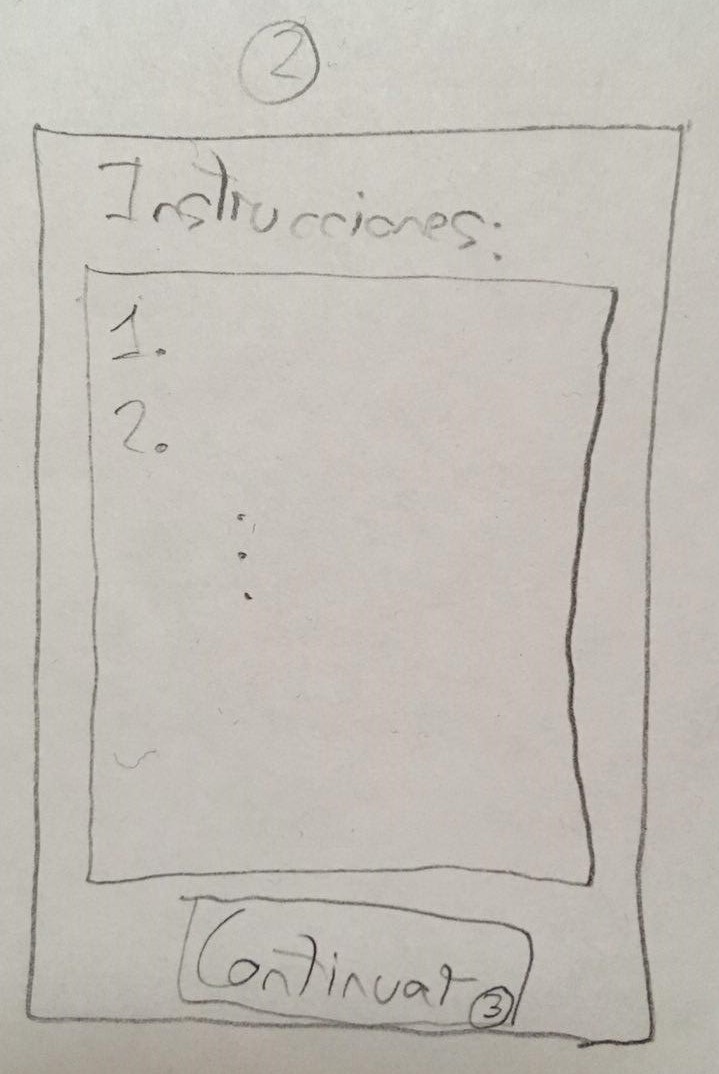
\includegraphics[scale=0.2]{b2}
  \caption{Imagen que muestra la interfaz de la pantalla de instrucciones del juego.\protect\footnotemark}
  \label{figura-b2}
\end{figure}

El resto de los bocetos se pueden encontrar en la sección \ref{bocetos} del Anexo.

\subsection{Pruebas heurísticas}
Se han realizado pruebas heurísticas de usabilidad sobre los bocetos diseñados, estas pruebas consisten en comprobar diferentes aspectos de la usabilidad de la aplicación en función de los doce principios de Nielsen \cite{nielsen}, dichas comprobaciones se llevarán a cabo por desarrolladores del equipo, que en este caso está formado por un solo desarrollador.

\begin{itemize}
  \item \textbf{Principio 1: Visibilidad del estado del sistema.}\\
  La puntuación es de 7, el usuario está bien informado de lo que ocurre actualmente en el sistema, se muestra siempre que es necesario el botón “home” o el botón “atrás”, pero se puede mejorar, por ejemplo, indicando que se están escaneando imágenes mientras mueves el dispositivo sobre el tablero.

  \item \textbf{Principio 2: Correspondencia entre el sistema y el mundo real.}\\
  La puntuación es de 10, las opciones en los menús están ordenadas de forma lógica y el lenguaje que el juego utiliza es un lenguaje común al usuario del juego.

  \item \textbf{Principio 3: Control y libertad del usuario.}\\
  La puntuación es de 7, ya que en la mayoría de pantallas el usuario es libre de ir hacia adelante o hacia atrás, pero en instrucciones el usuario puede avanzar al juego pero no volver a la pantalla de inicio. Además, como se puede ver en la pantalla 6, para hacer apuntes, el botón de retroceso está en la zona derecha de la pantalla, pudiendo confundir esto al usuario, ya que es una función de retroceso no de avance.

  \item \textbf{Principio 4: Consistencia y estándares.}\\
  La puntuación es de 7, ya que es bastante consistente, pero en la pantalla que indica el ganador aparece el botón “home” como en otras pantallas, pero se muestra en una posición distinta, lo que resulta confuso al usuario habría que moverlo a la posición que ocupa siempre o utilizar otro botón.

  \item \textbf{Principio 5: Prevención de errores.}\\
  La puntuación es de 10, el diseño es bastante cuidadoso para la prevención de errores y el correcto tratamiento de estos.

  \item \textbf{Principio 6: Minimizar la carga de memoria del usuario.}\\
  La puntuación es de 10, el usuario no necesita recordar nada en ningún momento, todo se muestra de forma apropiada para que no suponga ninguna memorización al usuario.

  \item \textbf{Principio 7: Personalización y atajos.}
  La puntuación es de 10, la aplicación no dispone de personalización o atajos, pero no son necesarios en esta, por lo que no afecta a la experiencia de usuario.

  \item \textbf{Principio 8: Eficiencia de uso y rendimiento.}
  La puntuación es de 8, la aplicación está bien optimizada para que al usuario le resulte sencillo y rápido llevar a cabo cualquier tarea, pero si es cierto que algunos botones que se utilizan con mucha frecuencia no están en las posiciones óptimas.

  \item \textbf{Principio 9: Estética y diseño minimalista.}
  La puntuación es de 10, la información que se muestra en la aplicación es la necesaria para que el usuario pueda jugar con la mejor experiencia de usuario posible, no hay exceso o falta de información.

  \item \textbf{Principio 10: Ayuda al usuario a reconocer, diagnosticar y recuperarse de errores.}
  La puntuación es de 10, ya que no hay posibilidad de que ocurran errores en el juego.

  \item \textbf{Principio 11: Ayuda y documentación.}
  La puntuación es de 10, ya que antes de comenzar cada partida se muestra al usuario unas instrucciones de cómo funciona el juego.

  \item \textbf{Principio 12: Interacción física y ergonomía.}
  La puntuación es de 10, ya que los botones son fácilmente diferenciables y están en una posición cómoda para el usuario, teniendo en cuenta que al ser un juego utilizará las dos manos para usar el dispositivo móvil.

\end{itemize}

\subsection{Pruebas de usabilidad}
Se han realizado pruebas de usabilidad con usuarios sobre los bocetos diseñados, estas pruebas consisten en poner al usuario en una determinada situación y solicitarle que realice una tarea, se observará como lo hace y se anotarán dificultades y comentarios, esto ayuda a solucionar problemas y mejorar la aplicación.\\

Se han realizado pruebas heurísticas de usabilidad sobre los bocetos diseñados, estas pruebas consisten en comprobar diferentes aspectos de la usabilidad de la aplicación en función de los diez principios de Nielsen \cite{nielsen}, dichas comprobaciones se llevarán a cabo por desarrolladores del equipo, que en este caso está formado por un solo desarrollador.

Las tablas que contienen la información obtenida en estas pruebas de usabilidad se encuentran en la sección \ref{tablas-usabilidad-bocetos} del Anexo.

\begin{itemize}
  \item \textbf{Usuario 1}

  \textbf{Pre Test}

  \begin{enumerate}
    \item Edad: 18
    \item Dispone de un dispositivo móvil: Sí
    \item Con qué frecuencia utiliza su dispositivo móvil: Varias veces al día
    \item Con qué frecuencia juega a juegos de mesa: Varias veces al año
    \item Con qué frecuencia juega a juegos en su móvil: Varias veces a la semana
  \end{enumerate}

  \textbf{Test}: Los resultados del test de usabilidad sobre el Usuario 1 se encuentran en la Tabla \ref{tabla-bocetos-usuario1}


  \item \textbf{Usuario 2}

  \textbf{Pre Test}

  \begin{enumerate}
    \item Edad: 57
    \item Dispone de un dispositivo móvil: Sí
    \item Con qué frecuencia utiliza su dispositivo móvil: Varias veces al día
    \item Con qué frecuencia juega a juegos de mesa: Varias veces al año
    \item Con qué frecuencia juega a juegos en su móvil: Varias veces al día
  \end{enumerate}

  \textbf{Test}: Los resultados del test de usabilidad sobre el Usuario 2 se encuentran en la Tabla \ref{tabla-bocetos-usuario2}


  \item \textbf{Usuario 3}

  \textbf{Pre Test}

  \begin{enumerate}
    \item Edad: 26
    \item Dispone de un dispositivo móvil: Sí
    \item Con qué frecuencia utiliza su dispositivo móvil: Varias veces al día
    \item Con qué frecuencia juega a juegos de mesa: Una vez al mes como máximo
    \item Con qué frecuencia juega a juegos en su móvil: Casi nunca
  \end{enumerate}

  \textbf{Test}: Los resultados del test de usabilidad sobre el Usuario 3 se encuentran en la Tabla \ref{tabla-bocetos-usuario3}

\end{itemize}

\subsection{Segunda iteración}
En esta iteración se ha creado el diagrama de clases del sistema haciendo uso del lenguaje UML, dicho diagrama de clases se puede consultar en el Apéndice \ref{apendice-diagrama-de-clases}.

Por otro lado, se han llevado a cabo los bocetos, que se pueden encontrar en el Apéndice \ref{bocetos}, esos nos servirán para crear un primer concepto de como serán las interfaces de las diferentes pantallas del juego.\\

También se llevaron a cabo pruebas heurísticas con el desarrollador, para comprobar los posibles errores y mejoras de los bocetos. Los resultados de estas pruebas se pueden encontrar en la \textbf{Entrega 1}.\\

Por último, se realizaron pruebas con usuarios, poniéndoles en situación se les indicaba la tarea que tenían que hacer, y se fueron apuntando los problemas que estos tenían, detectando así elementos que mejorar en los bocetos. Los resultados de estas pruebas de usabilidad se encuentran en las Tablas \ref{tabla-bocetos-usuario1}, \ref{tabla-bocetos-usuario2} y \ref{tabla-bocetos-usuario3}.\\

Con toda la información obtenida de la realización de los bocetos y pruebas de usuario se han modificado aspectos del GDD, adaptando el funcionamiento del juego a las necesidades de los jugadores, y ajustando los perfiles de forma más realista al de los posibles futuros jugadores del juego. El documento de diseño del videojuego se puede encontrar en el Apéndice \ref{documento-diseño-videojuegos}.

\subsection{Conclusiones}
Durante las pruebas de usabilidad pruebas hemos podido comprobar que la interfaz de la aplicación es amigable para los usuarios, que si bien han detectado algunos fallos, que serán solventados en el desarrollo del juego, por lo general han sabido realizar todas las tareas sin dificultad, desenvolviéndose con rapidez.\\

También se ha podido comprobar el interés de los usuarios por el funcionamiento de la realidad aumentada, resultándoles algo sorprendente y que sin duda tenían ganas de probar en las siguientes pruebas de usabilidad, lo que denota la esperada expectación de los usuarios de juegos y en general de dispositivos móviles sobre la realidad aumentada y las novedosas experiencias que esta aportará al ámbito de los dispositivos móviles.

\section{Entrega 2}
En esta entrega se ha completado la pantalla inicial que permite seleccionar los personajes de los jugadores, la pantalla de instrucciones que explica el funcionamiento del juego y la pantalla de juego en la que se podrá escanear el tablero y se mostrarán los modelos 3D que se utilizarán en el juego sobre dicho tablero.\\

En la Figura \ref{figura-inicial-1} se puede observar la pantalla de inicio sin personajes seleccionados.

\begin{figure}[h]
  \centering
  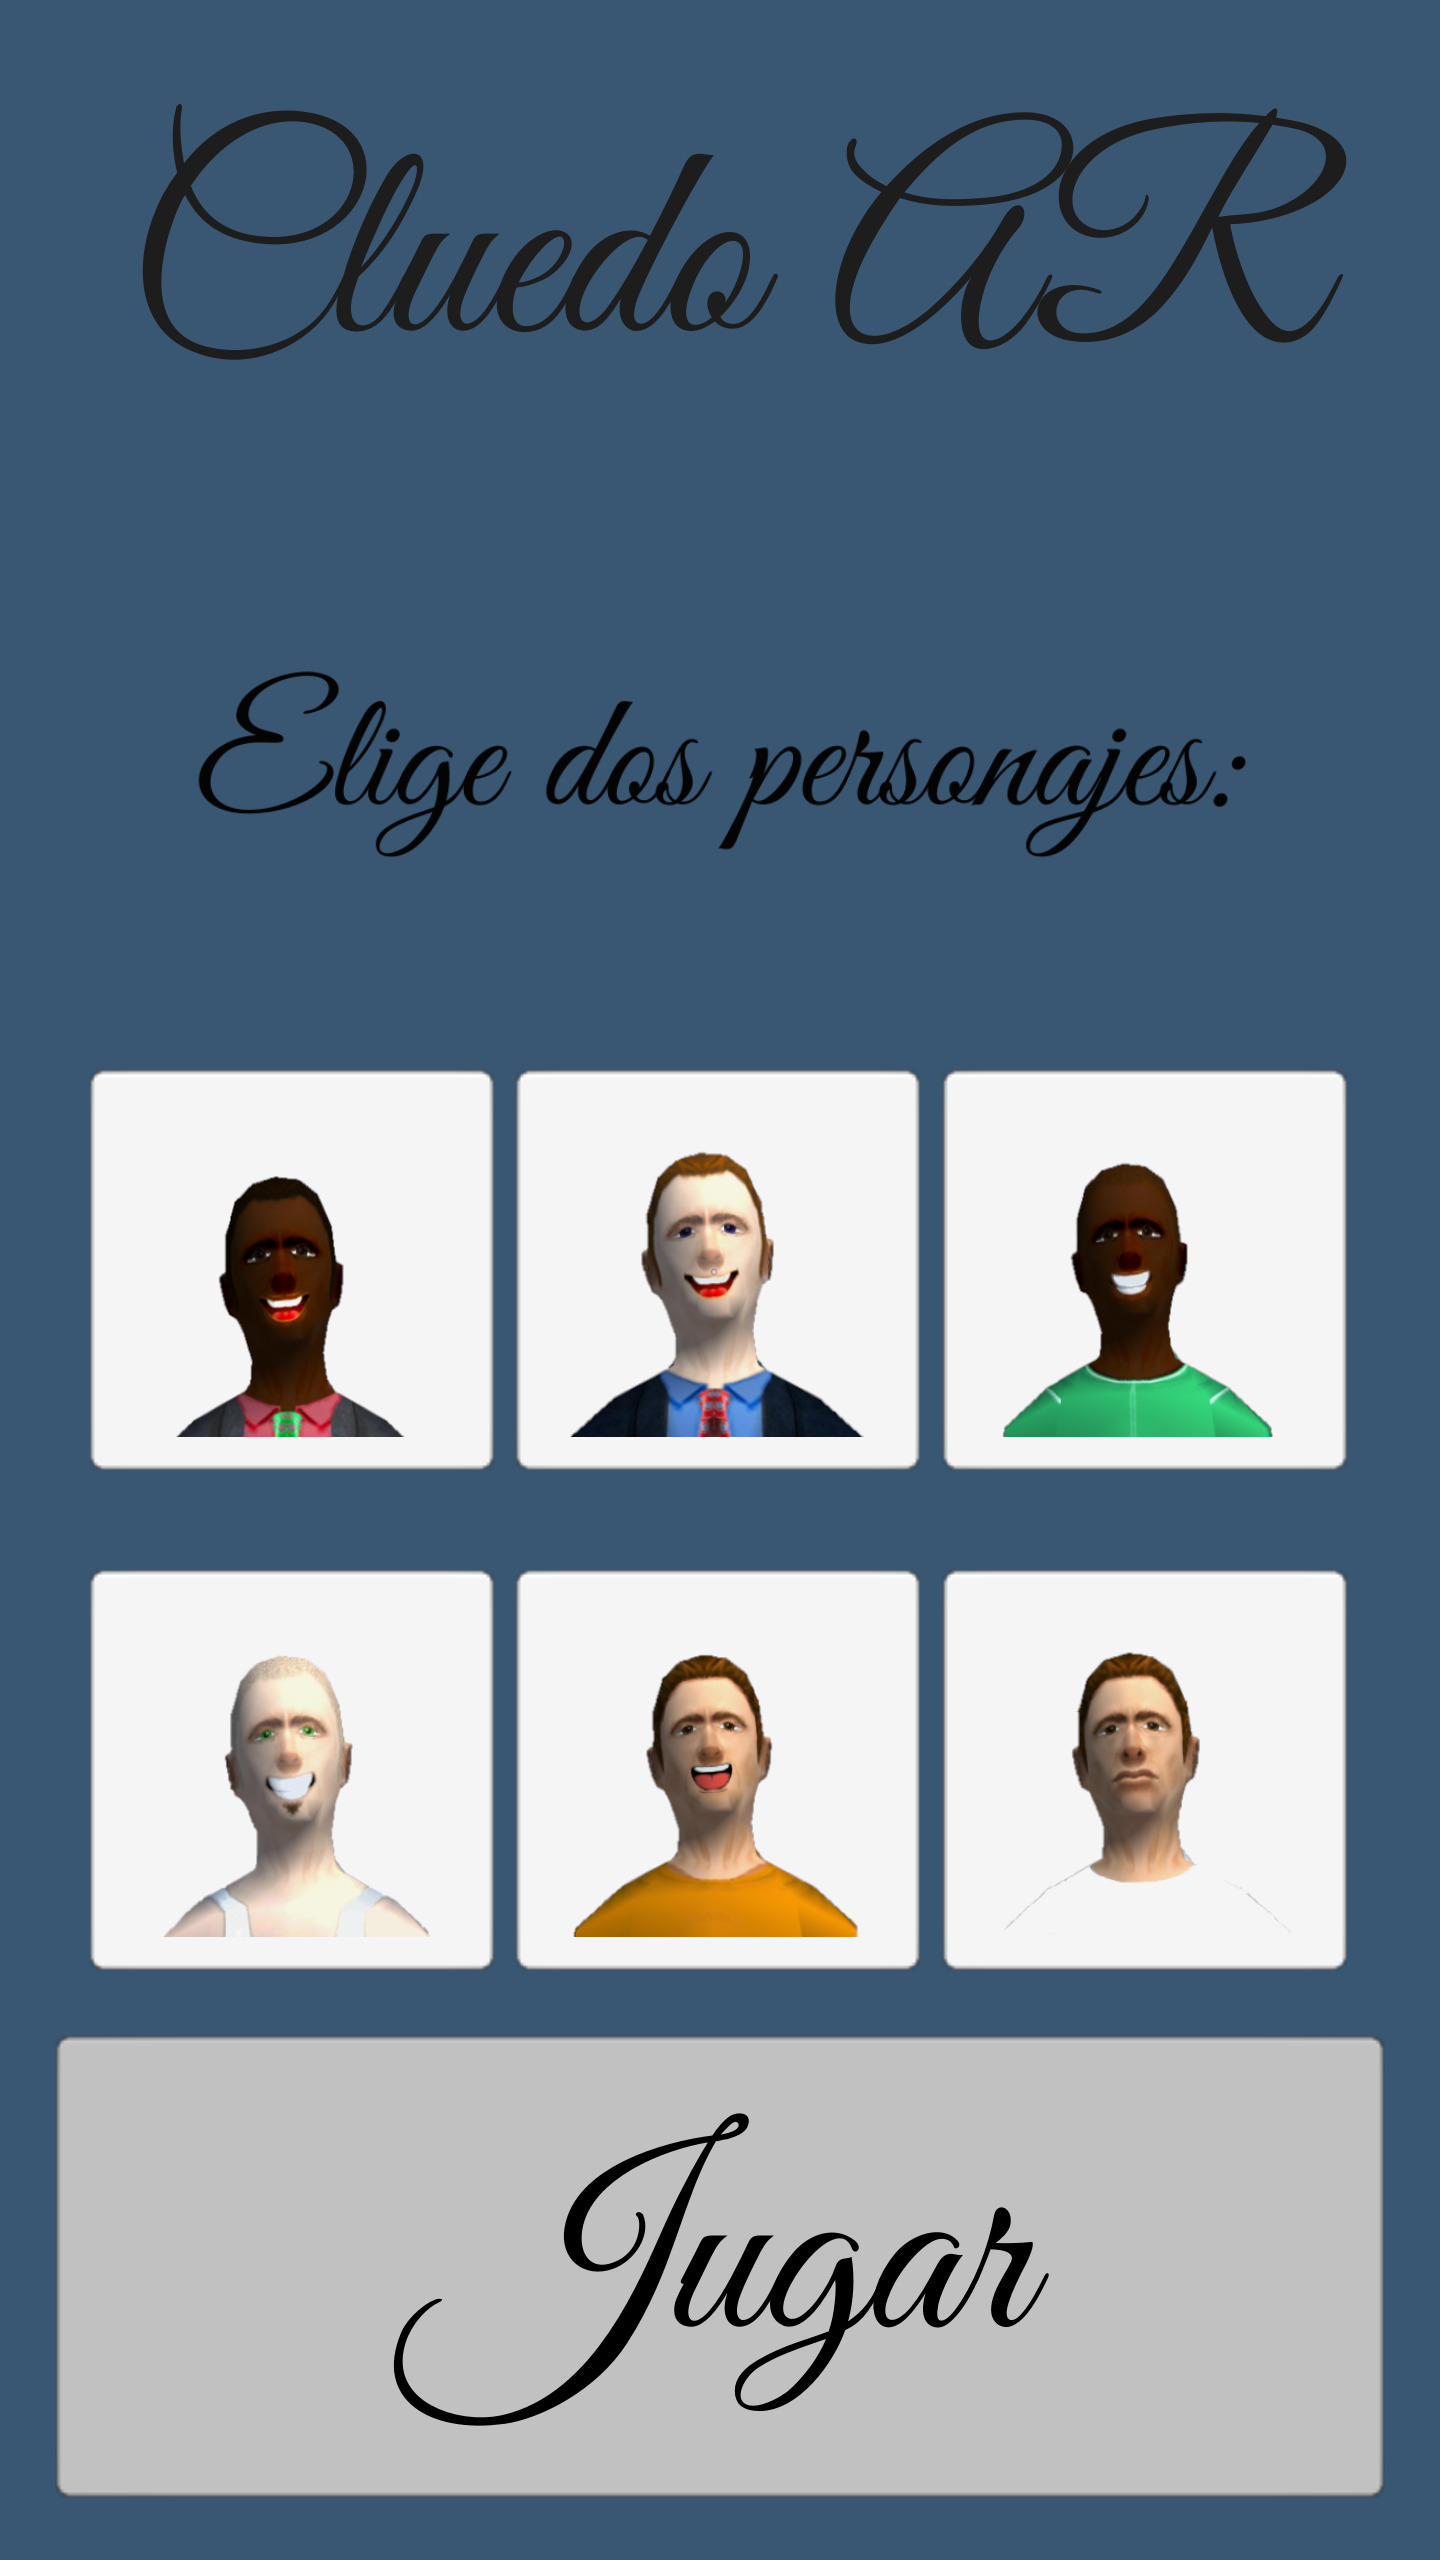
\includegraphics[scale=0.07]{inicial-1}
  \caption{Imagen que muestra la pantalla inicial sin personajes seleccionados.}
  \label{figura-inicial-1}
\end{figure}

\newpage

Mientras que en la Figura \ref{figura-inicial-2} se puede observar la pantalla de inicio con personajes seleccionados y por tanto el botón de jugar activo.

\begin{figure}[h]
  \centering
  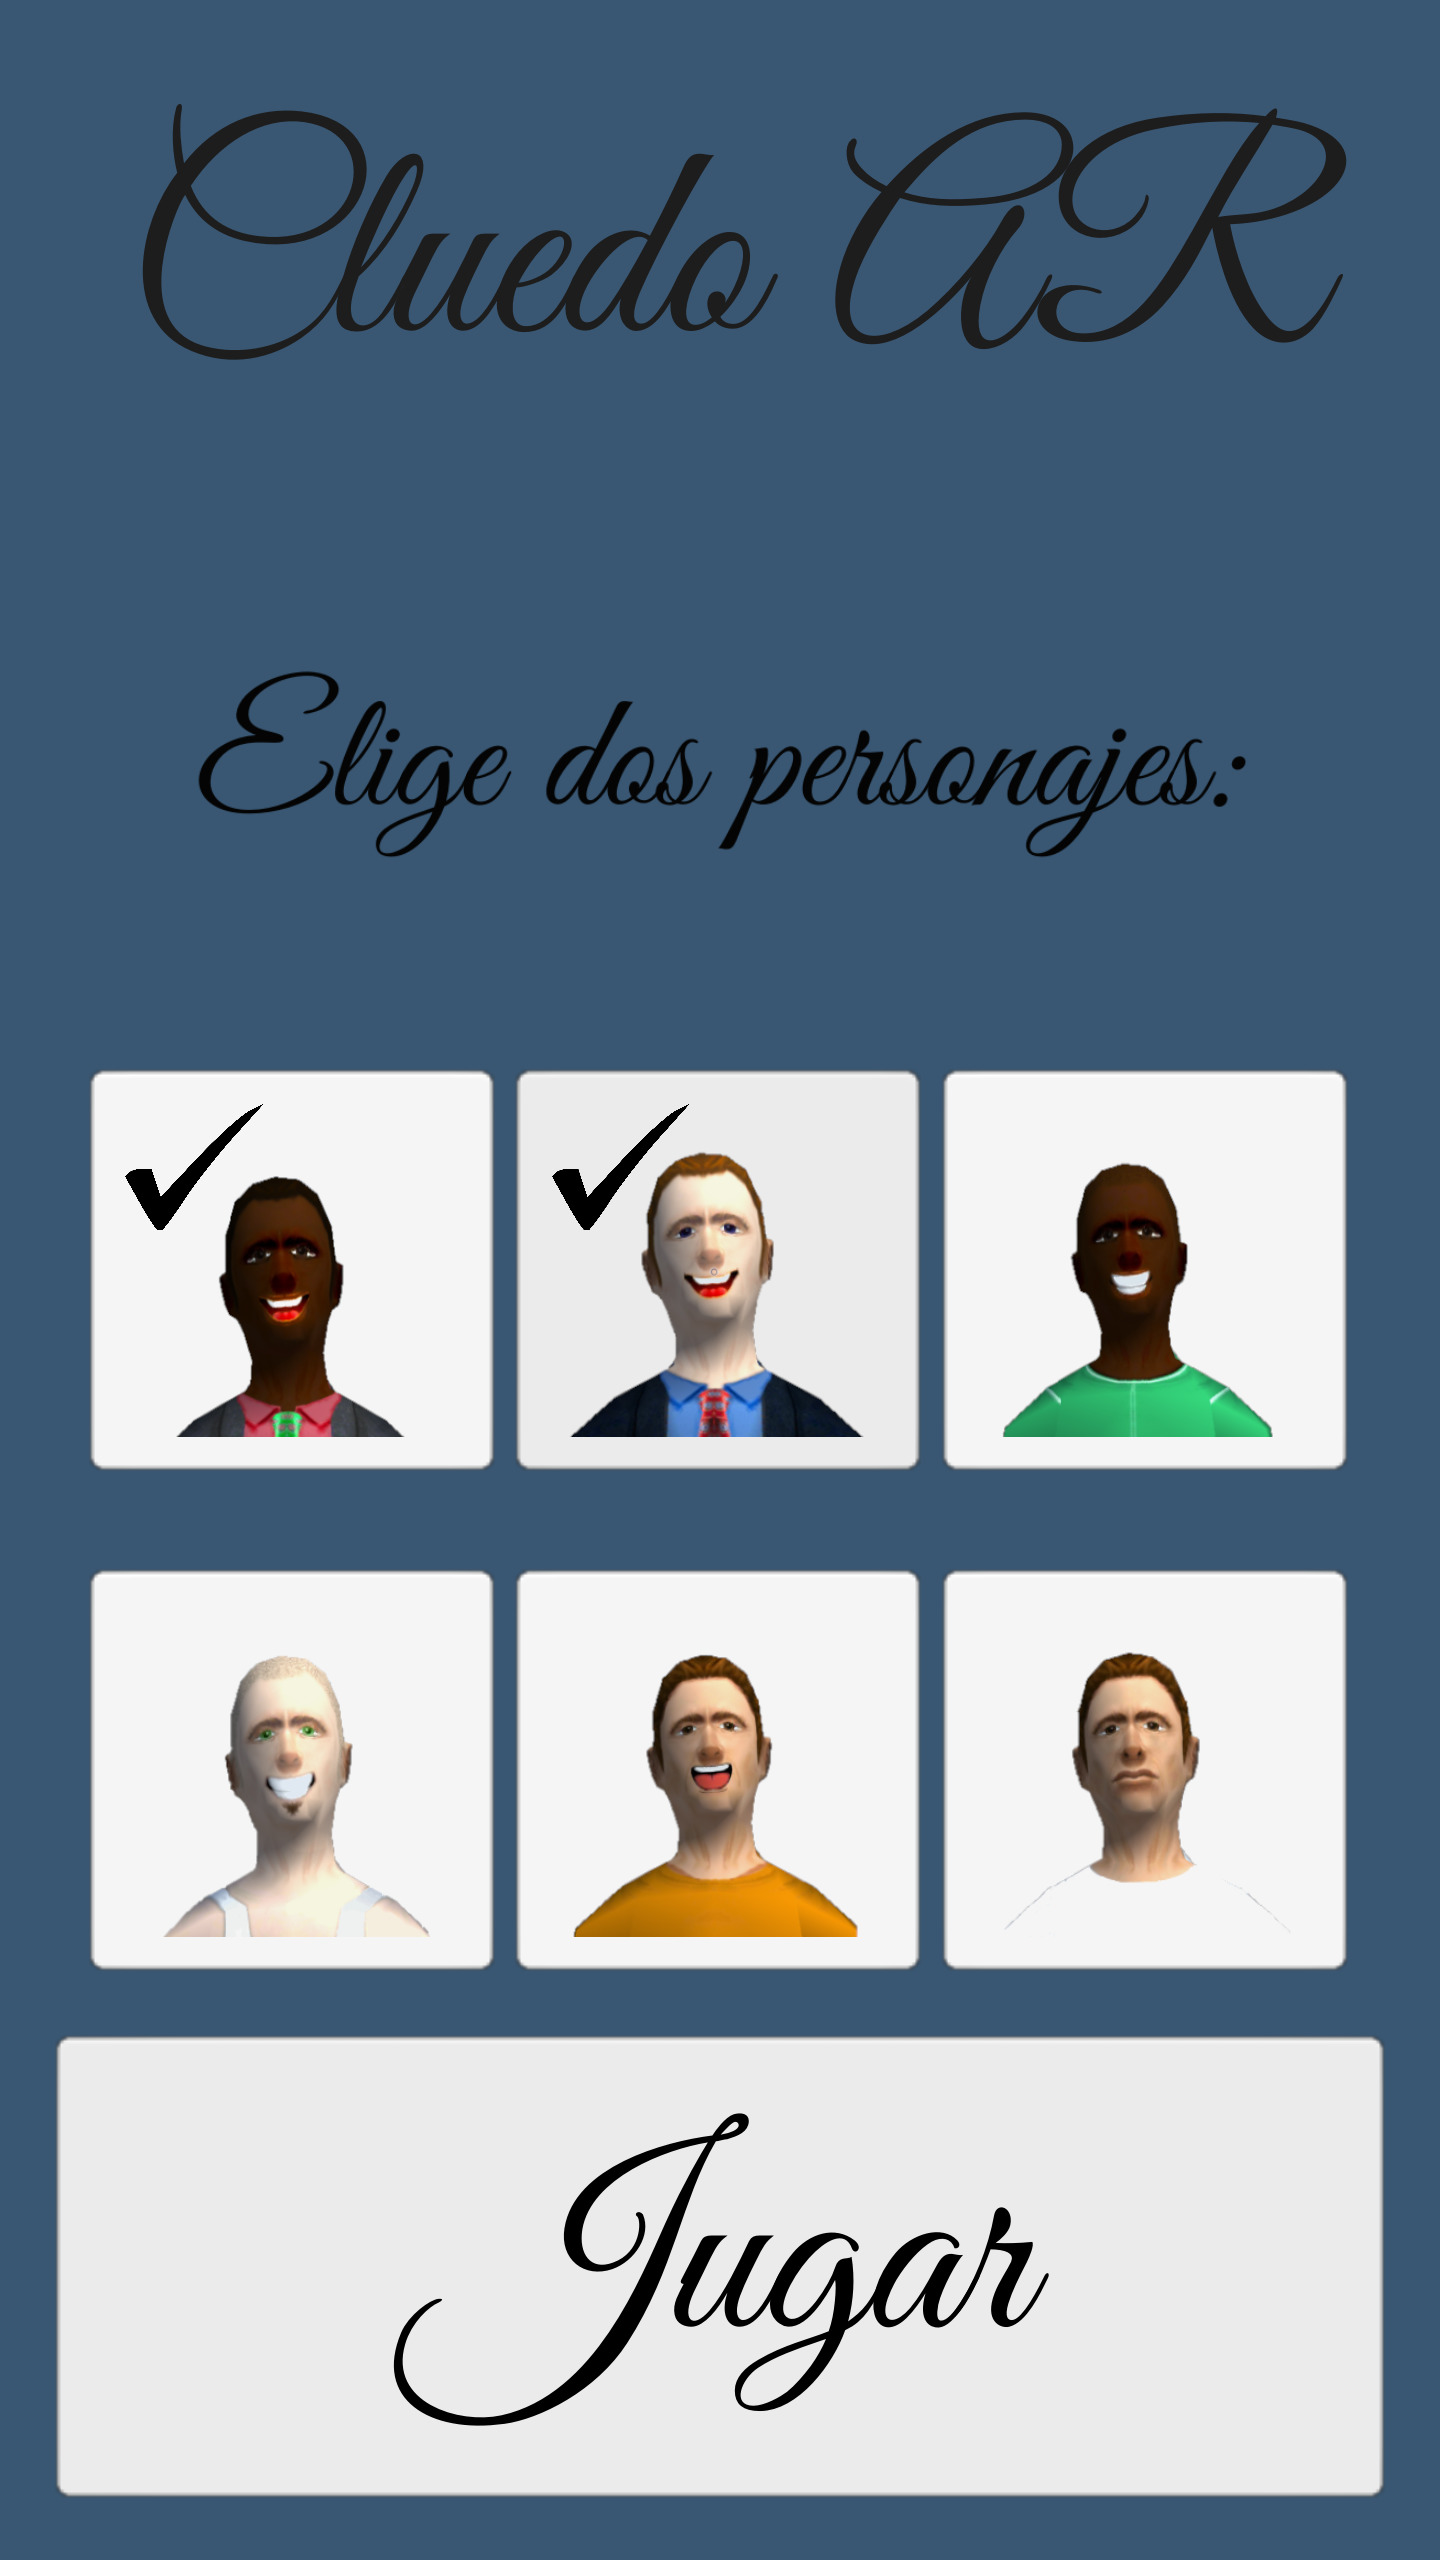
\includegraphics[scale=0.07]{inicial-2}
  \caption{Imagen que muestra la pantalla inicial con personajes seleccionados.}
  \label{figura-inicial-2}
\end{figure}

\newpage

En la Figura \ref{figura-instrucciones} se puede la pantalla de instrucciones.

\begin{figure}[h]
  \centering
  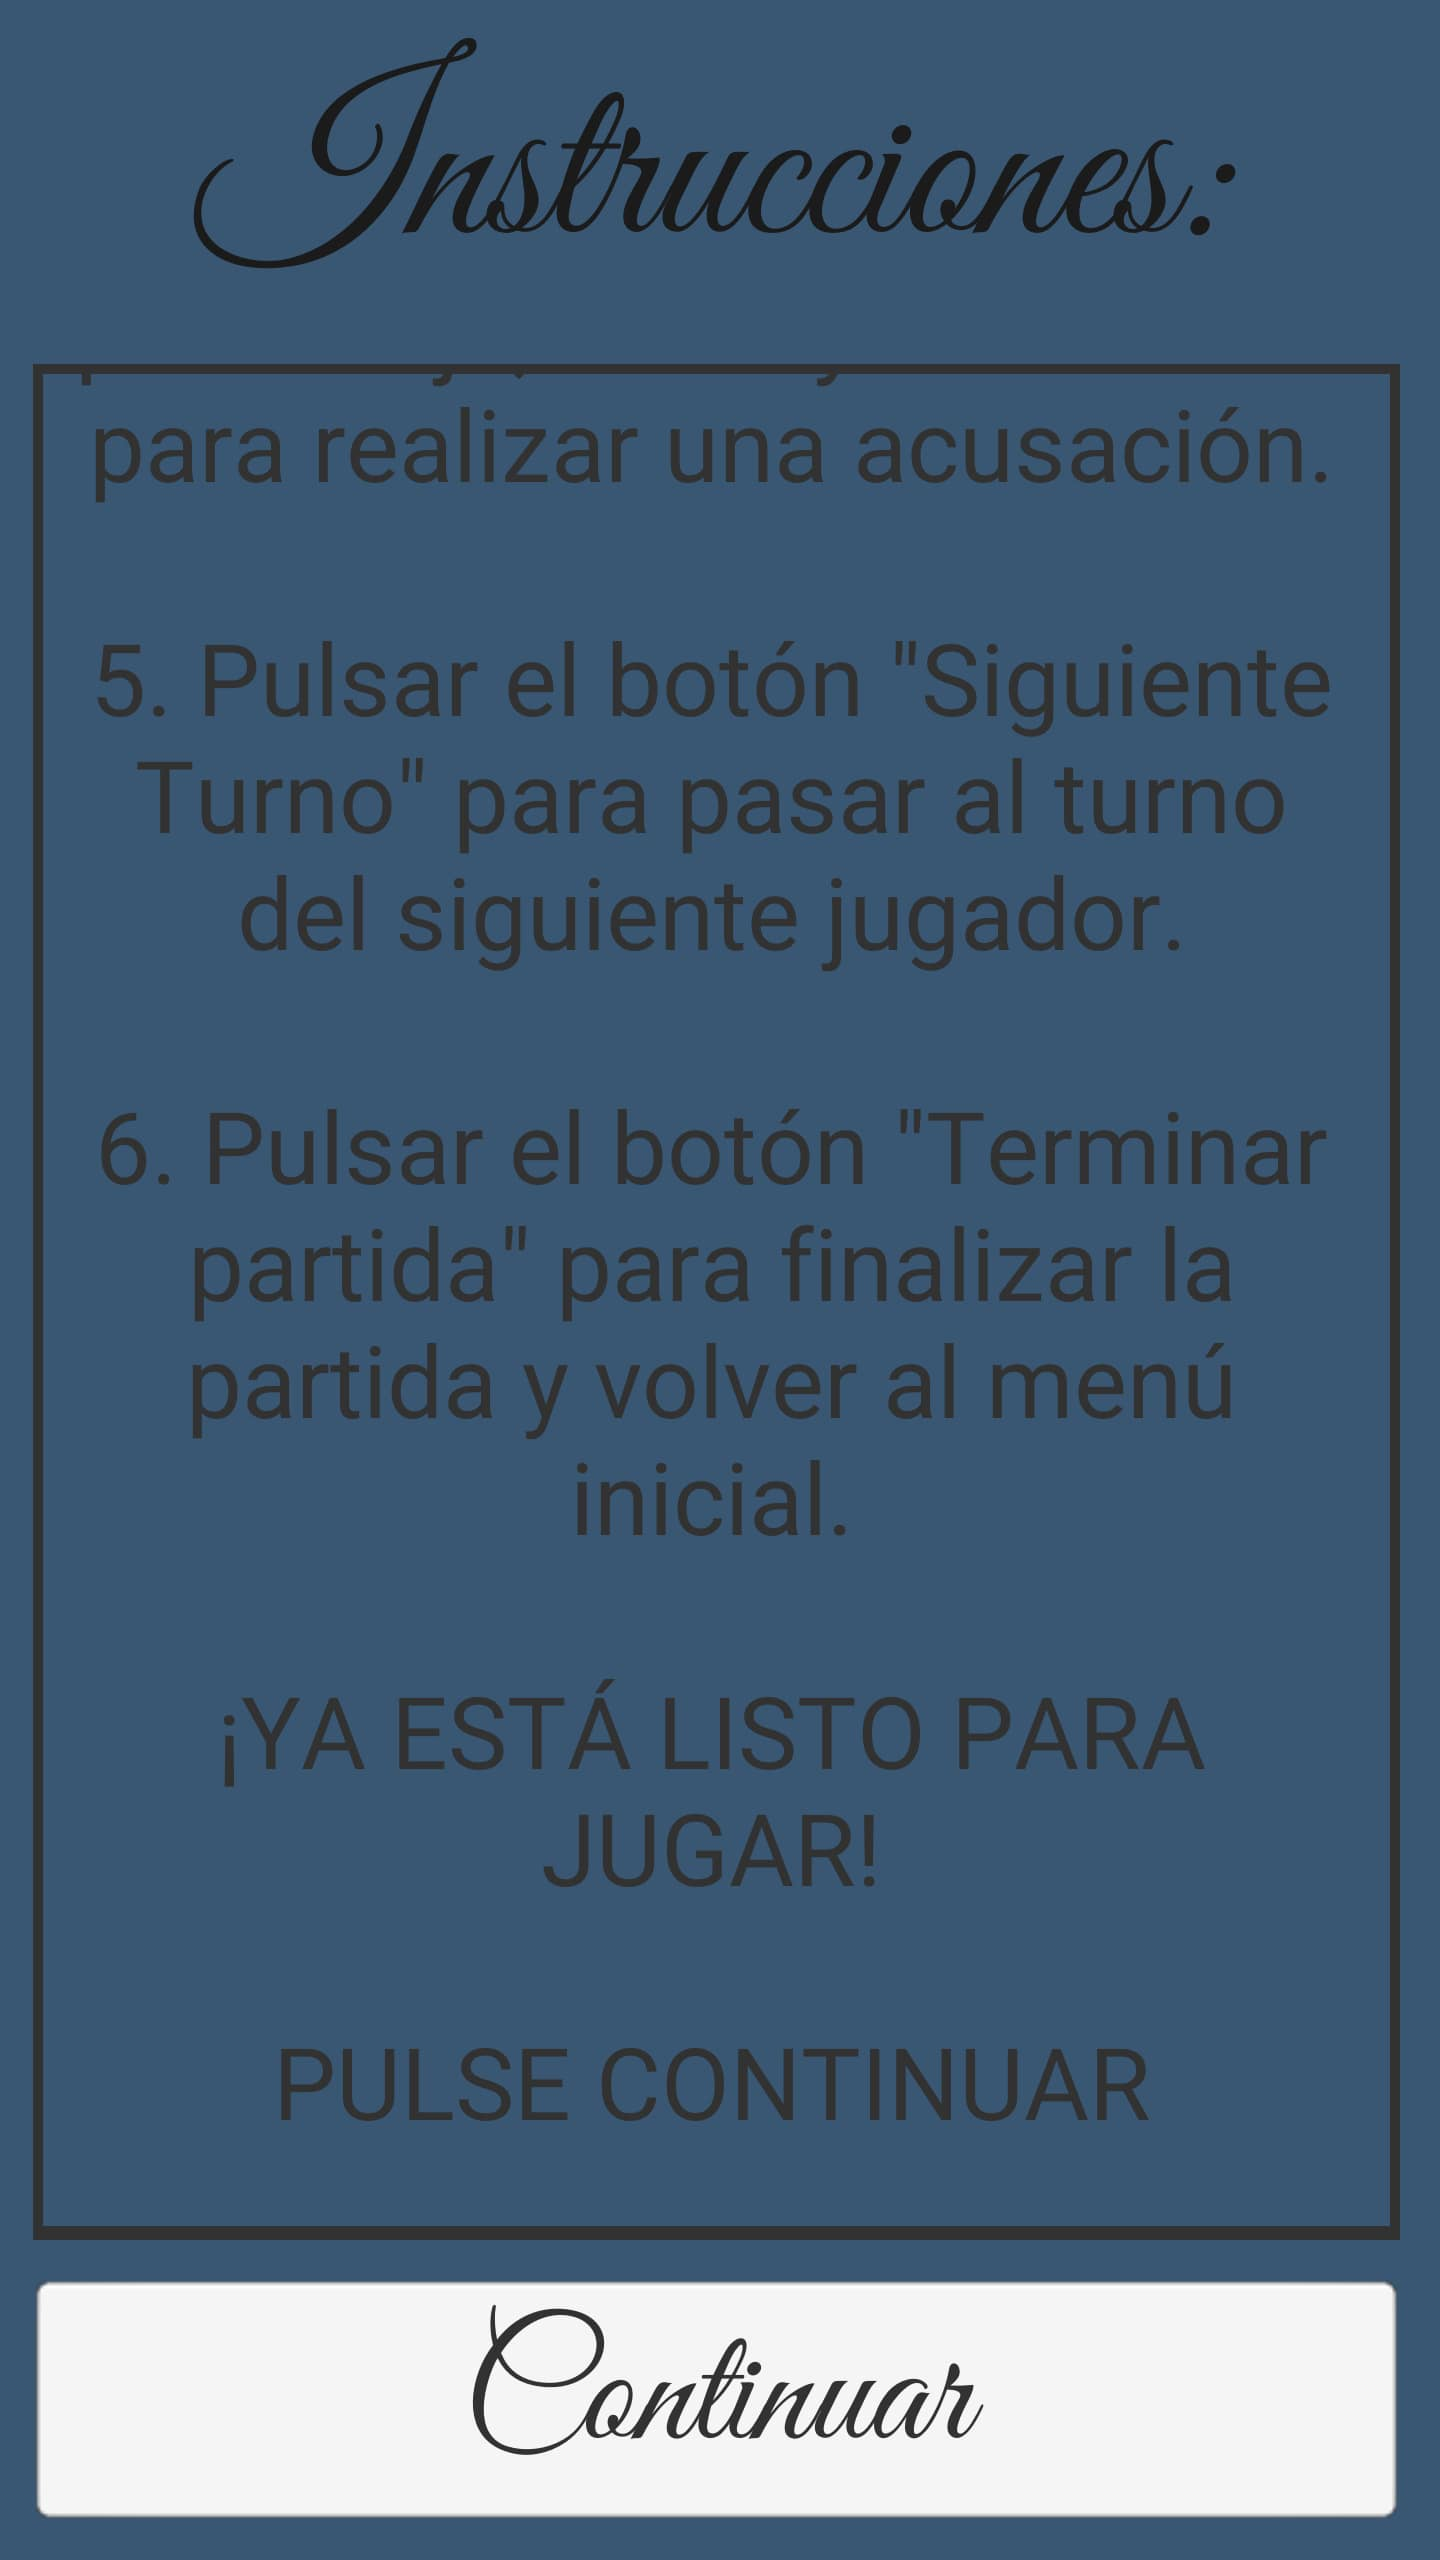
\includegraphics[scale=0.07]{instrucciones}
  \caption{Imagen que muestra la pantalla de instrucciones.}
  \label{figura-instrucciones}
\end{figure}


En la Figura \ref{figura-juego-1} se puede observar la pantalla de juego en con el tablero escaneado, mientras que en la Figura \ref{figura-juego-2} se puede observar mas de cerca como se sitúan los elementos sobre el tablero, y sobre cada habitación.

\begin{figure}[h]
  \centering
  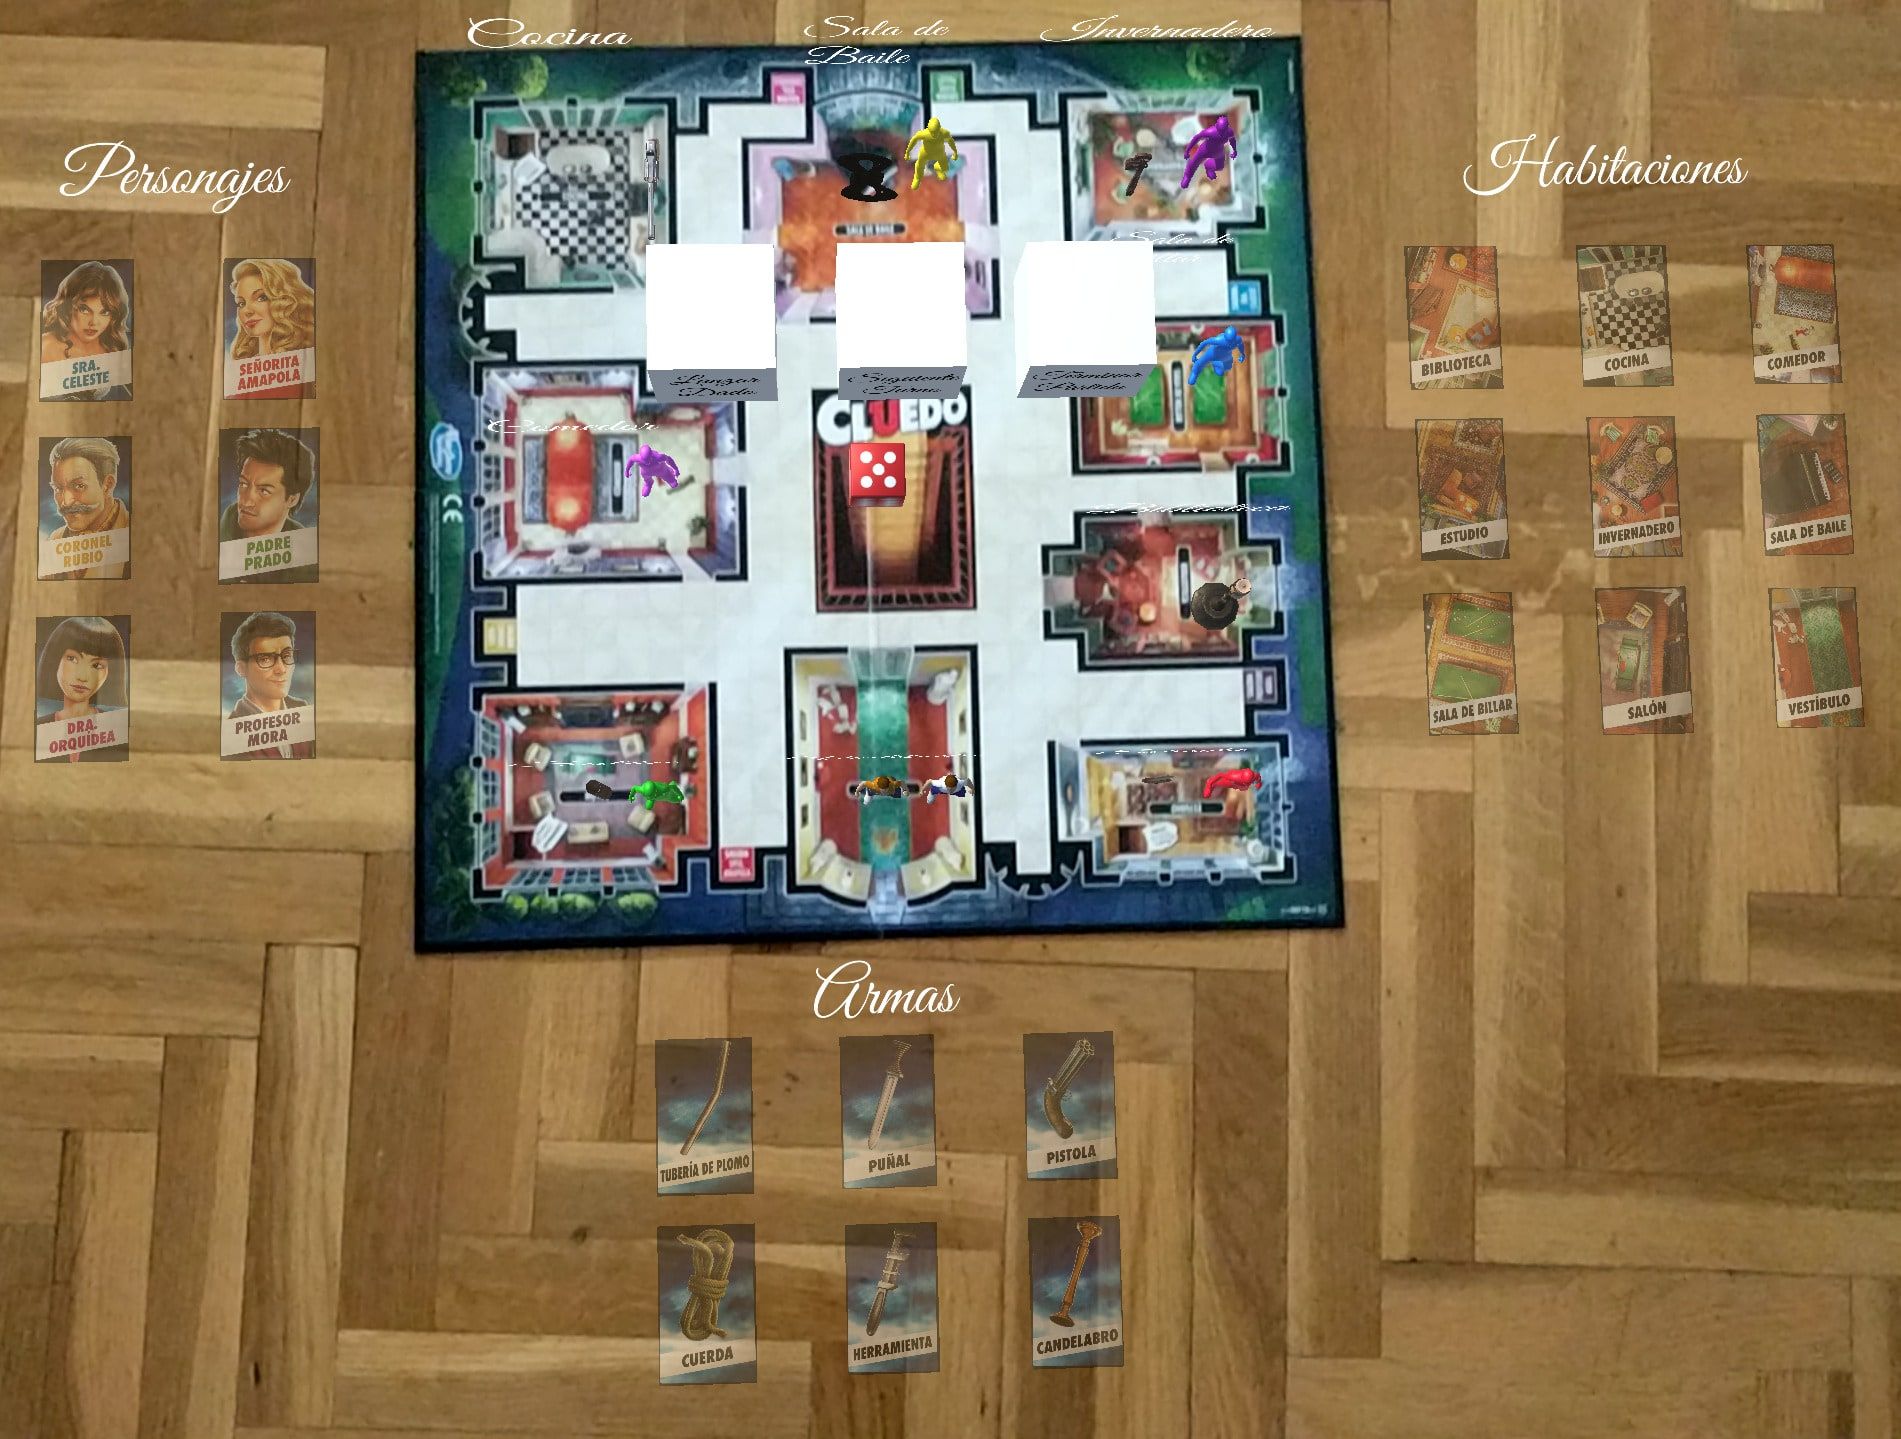
\includegraphics[scale=0.13]{juego-1}
  \caption{Imagen que muestra la pantalla de juego con el tablero escaneado.}
  \label{figura-juego-1}
\end{figure}

\begin{figure}[h]
  \centering
  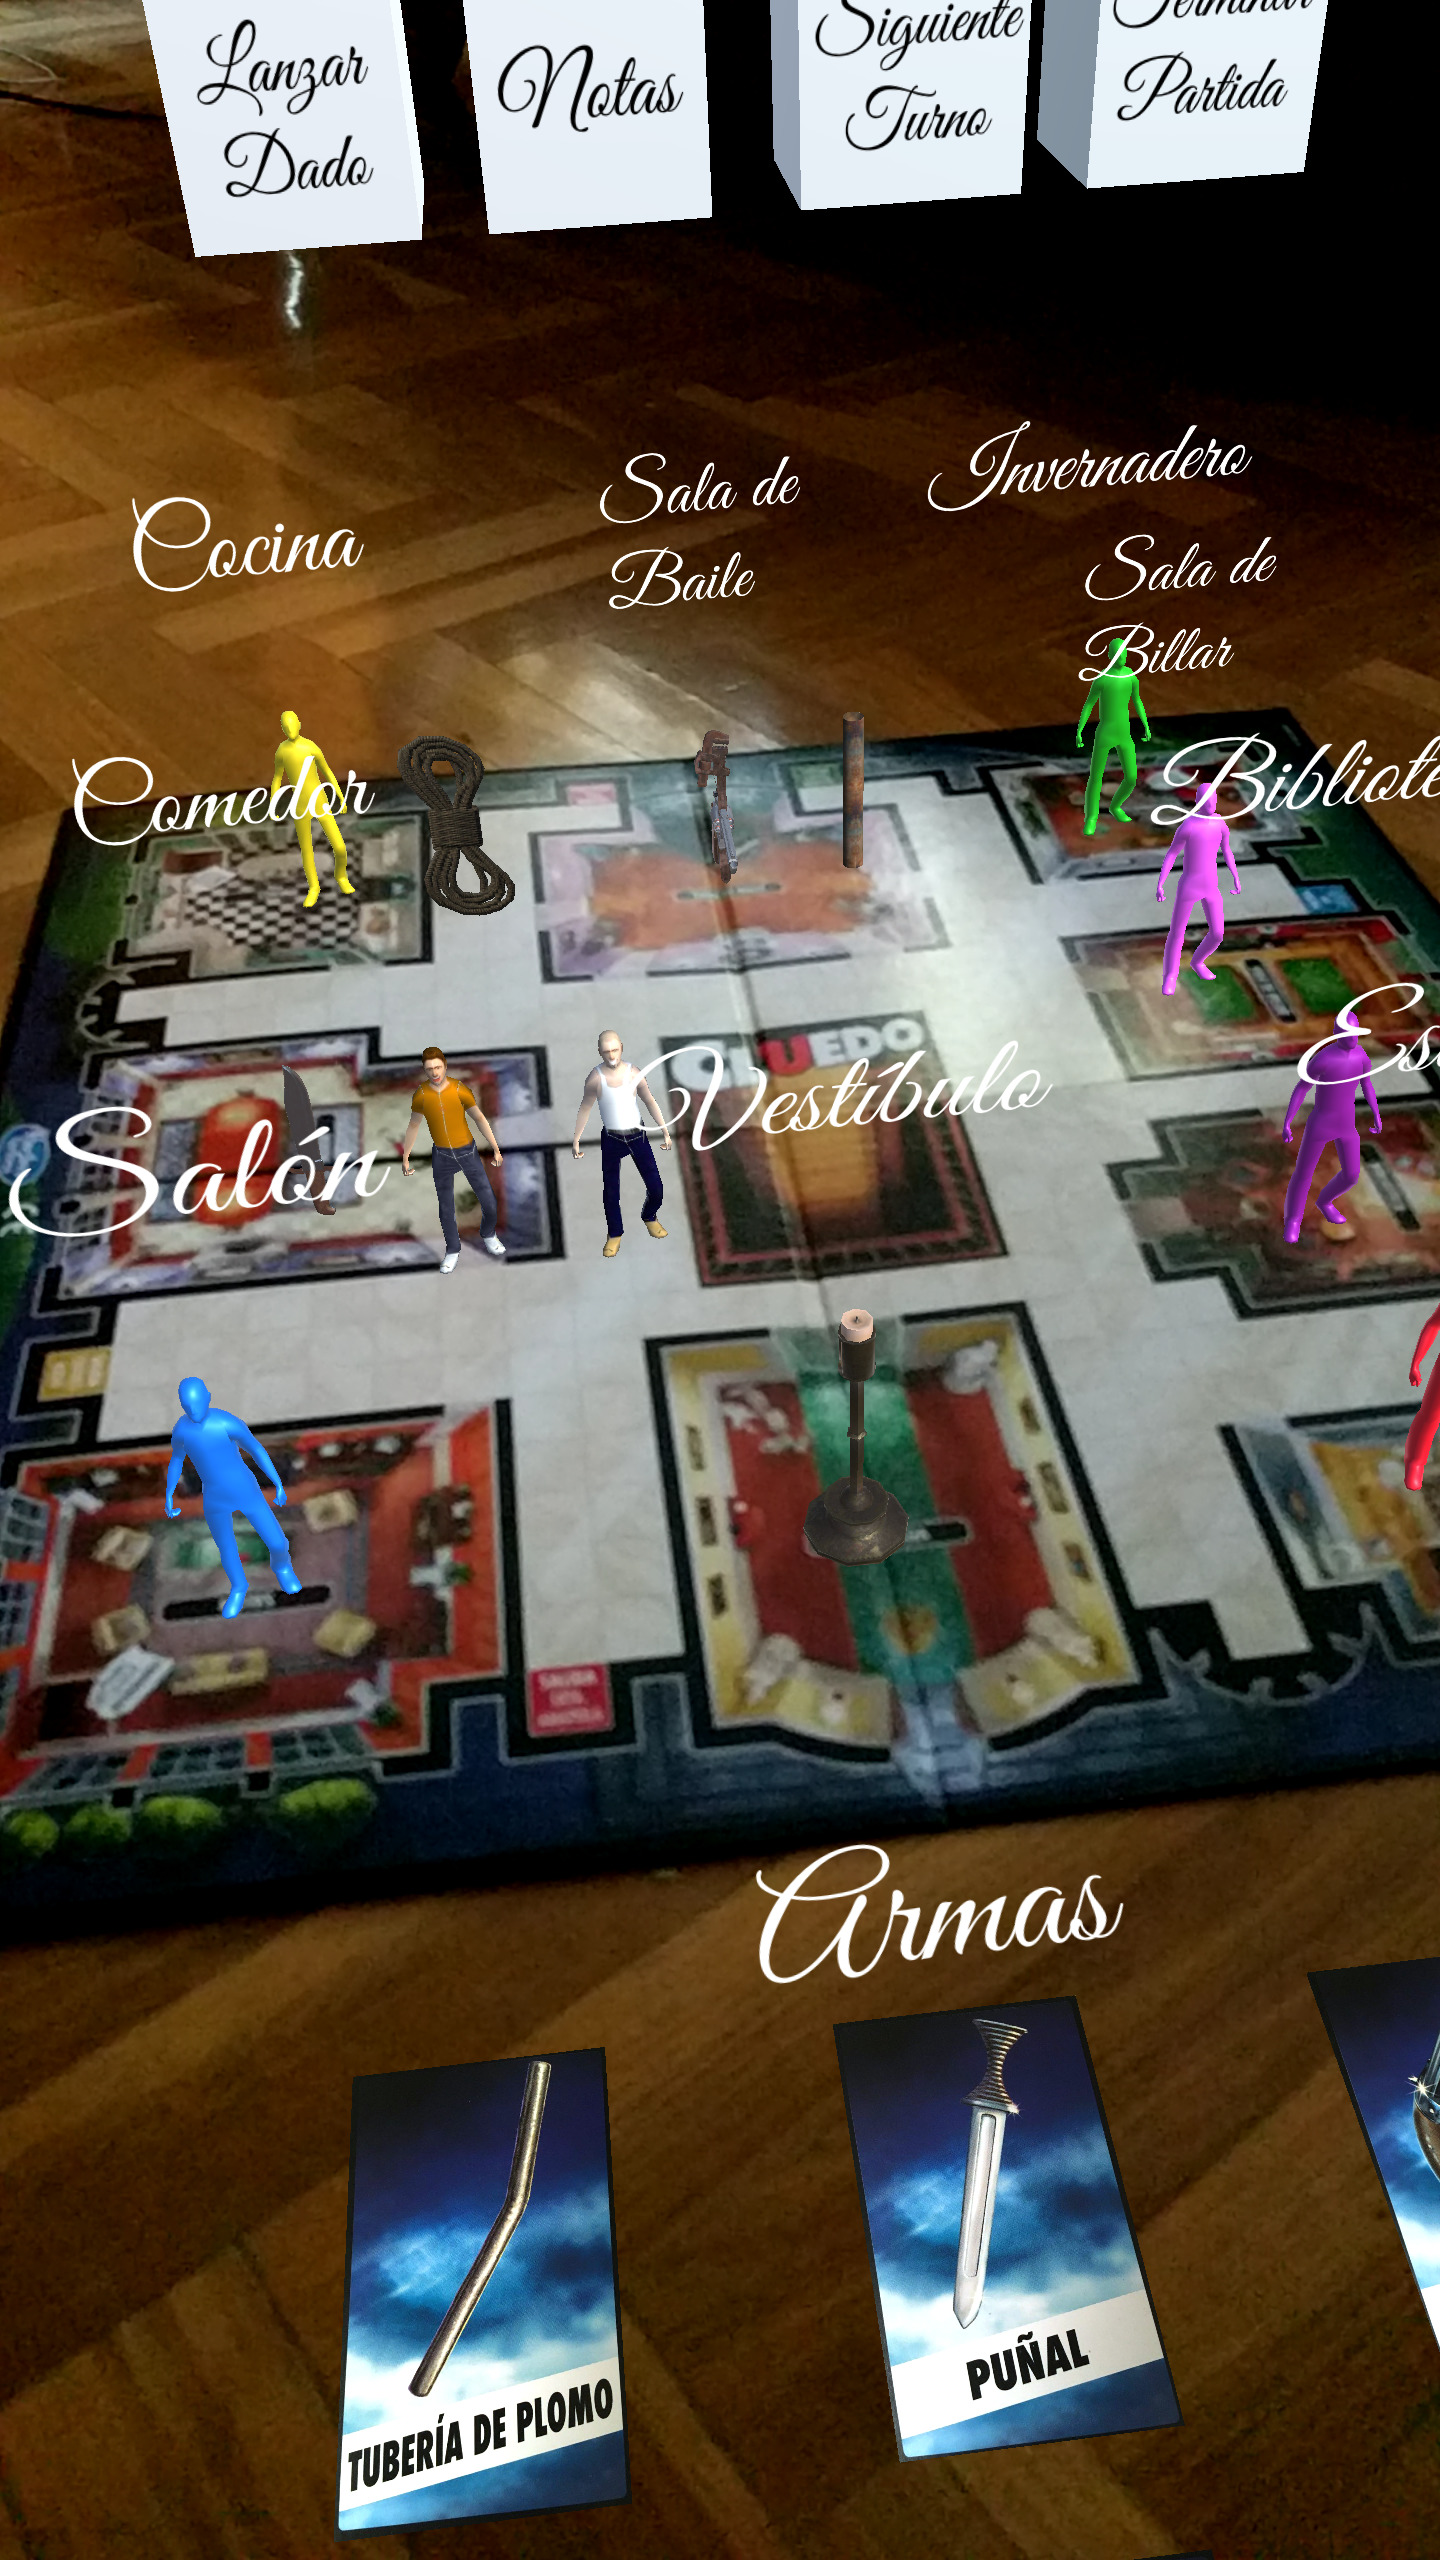
\includegraphics[scale=0.08]{juego-2}
  \caption{Imagen que muestra la pantalla de juego mas de cerca mostrando mas detalles.}
  \label{figura-juego-2}
\end{figure}

\FloatBarrier


\subsection{Tercera iteración}
En esta iteración se han llevado a cabo las historias de usuario \ref{tabla-hu1}, \ref{tabla-hu2} y \ref{tabla-hu3}.\\

En rasgos mas generales, en esta iteración se ha llevado a cabo la pantalla inicial del juego y la pantalla de instrucciones, cuyo resultado se muestra en la \textbf{Entrega 2}.


\subsection{Cuarta iteración}
En esta iteración se ha llevado a cabo la historia de usuario \ref{tabla-hu4}.\\

En rasgos mas generales, en esta iteración se ha llevado a cabo la pantalla de juego que es la pantalla central sobre la que se desarrollará el juego, ya que es la que puede escanear el mundo real, el resultado se muestra en la \textbf{Entrega 2}.\\

Por último, se realizaron pruebas con usuarios, poniéndoles en situación se les indicaba la tarea que tenían que hacer, y se fueron apuntando los problemas que estos tenían, detectando así elementos que mejorar en las pantallas de la aplicación realizadas en esta entrega. Los resultados de estas pruebas de usabilidad se encuentran en las Tablas \ref{tabla-entrega-2-usuario1}, \ref{tabla-entrega-2-usuario2} y \ref{tabla-entrega-2-usuario3}.

\subsection{Conclusiones}
Tras la realización de esta entrega se concluye que el proyecto avanza de forma favorable, todas las tareas se han llevado a cabo dentro de plazo y no han surgido grandes problemas.\\

Por otro lado, en las pruebas de usabilidad se comprueba que una vez los usuarios realizan las tareas en el dispositivo móvil en lugar de en los bocetos lo hacen con mas facilidad, ninguno de ellos muestra grandes dificultades a la hora de realizar las tareas solicitadas, por lo que se concluye que el diseño de las pantallas llevadas a cabo en esta entrega se ha realizado de forma exitosa.

\section{Entrega 3}
En esta entrega se ha completado la funcionalidad de lanzar los dados, y por tanto que se pueda mover al personaje a otra habitación, la funcionalidad de realizar una anotación y la funcionalidad de realizar una acusación. También se ha creado la pantalla de terminar partida, para complementar el funcionamiento de la acusación, de forma que si esta es correcta se finalice el juego y se indique el ganador.\\

En la Figura \ref{figura-dado-1} se pueden observar los elementos que se muestran tras lanzar los dados, se muestra el resultado obtenido del dado y las habitaciones a las que el usuario puede desplazarse.

\begin{figure}[h]
  \centering
  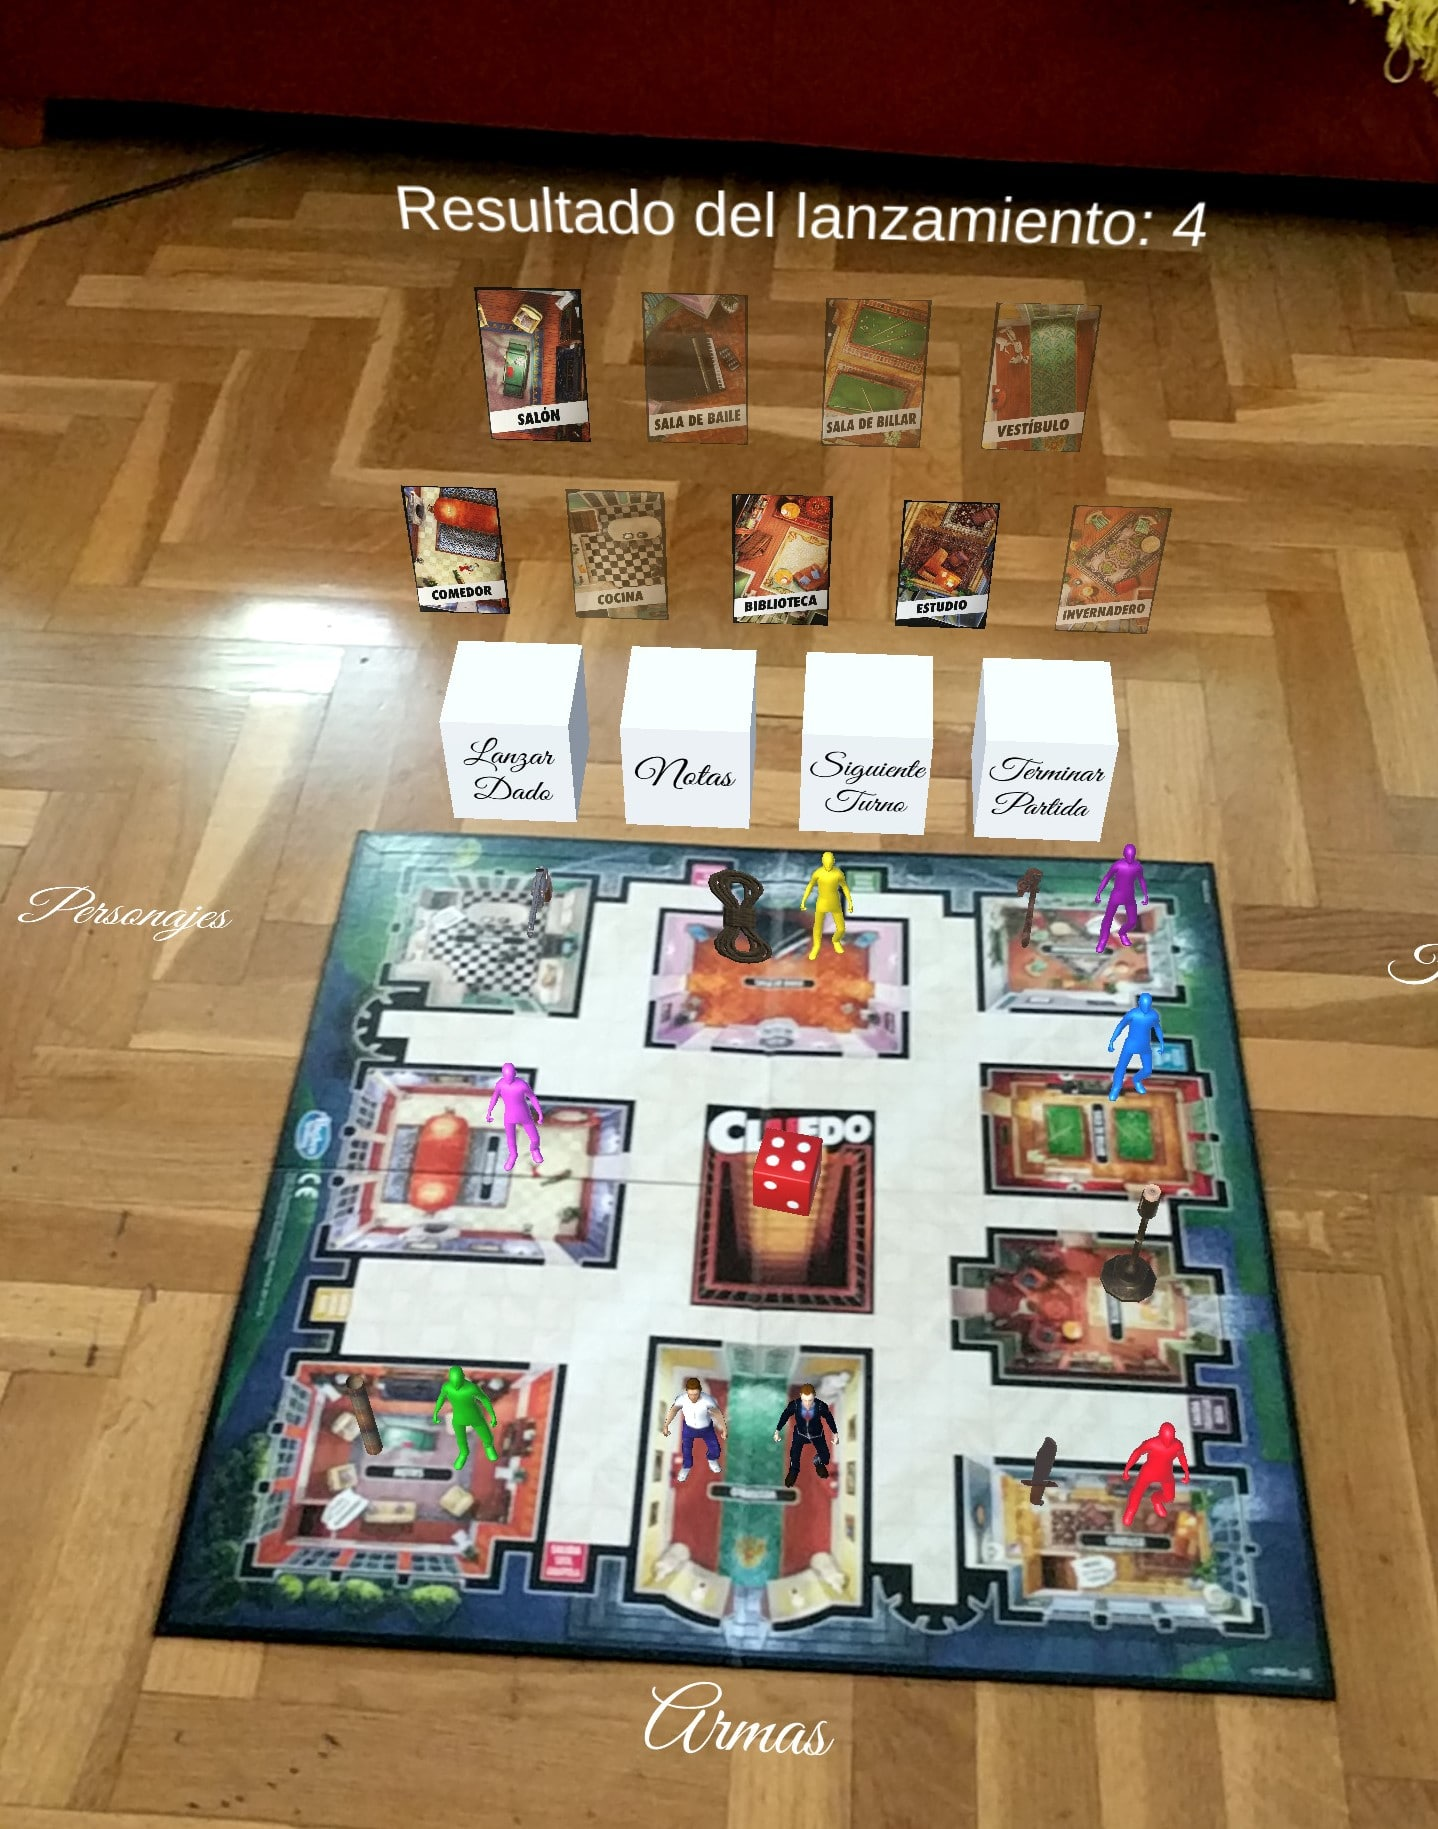
\includegraphics[scale=0.17]{dice-2}
  \caption{Imagen que muestra los elementos que el juego muestra tras lanzar los dados.}
  \label{figura-dado-1}
\end{figure}

\newpage

En la Figura \ref{figura-notas-1} se pueden observar los elementos que se muestran tras pulsar el botón de "Notas", se mostrarán las cartas diferenciadas por personajes, armas y habitaciones.

\begin{figure}[h]
  \centering
  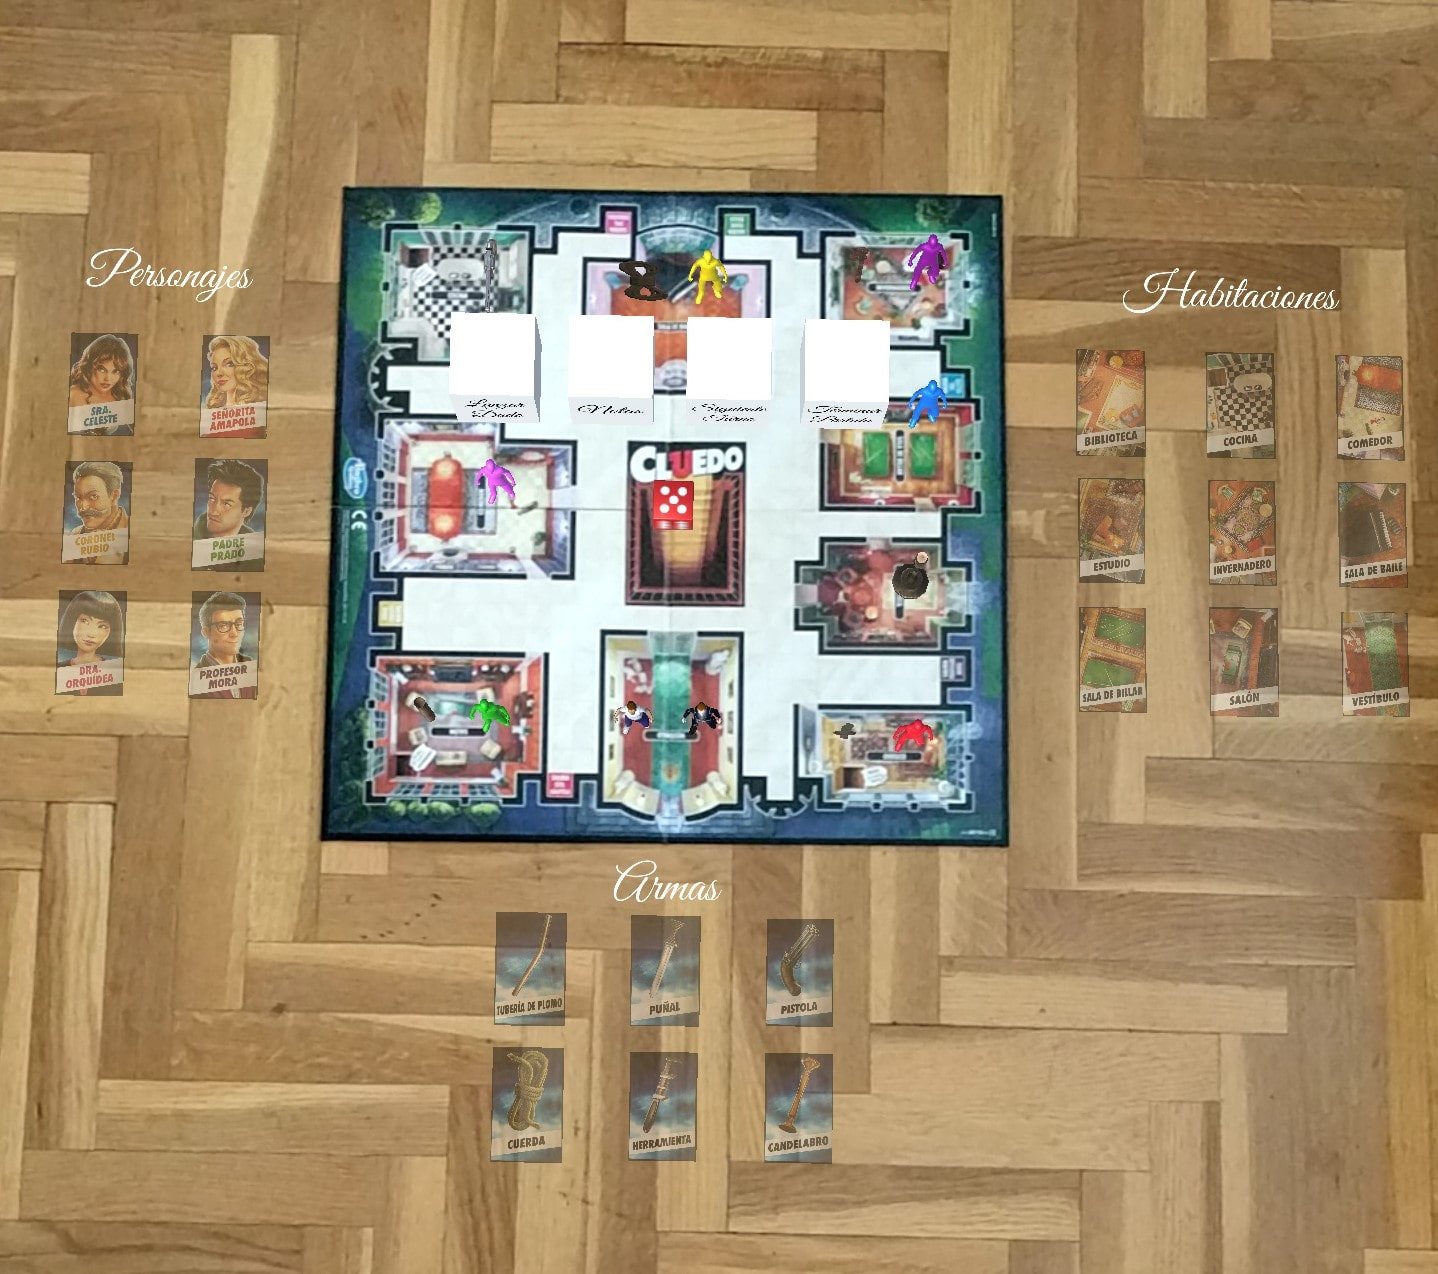
\includegraphics[scale=0.25]{notes-2}
  \caption{Imagen que muestra las cartas una vez pulsado el botón de notas.}
  \label{figura-notas-1}
\end{figure}

\newpage

En la Figura \ref{figura-notas-2} se pueden observar las cartas de armas en las que algunas están tachadas y otras no, lo que se consigue pulsando en ellas.

\begin{figure}[h]
  \centering
  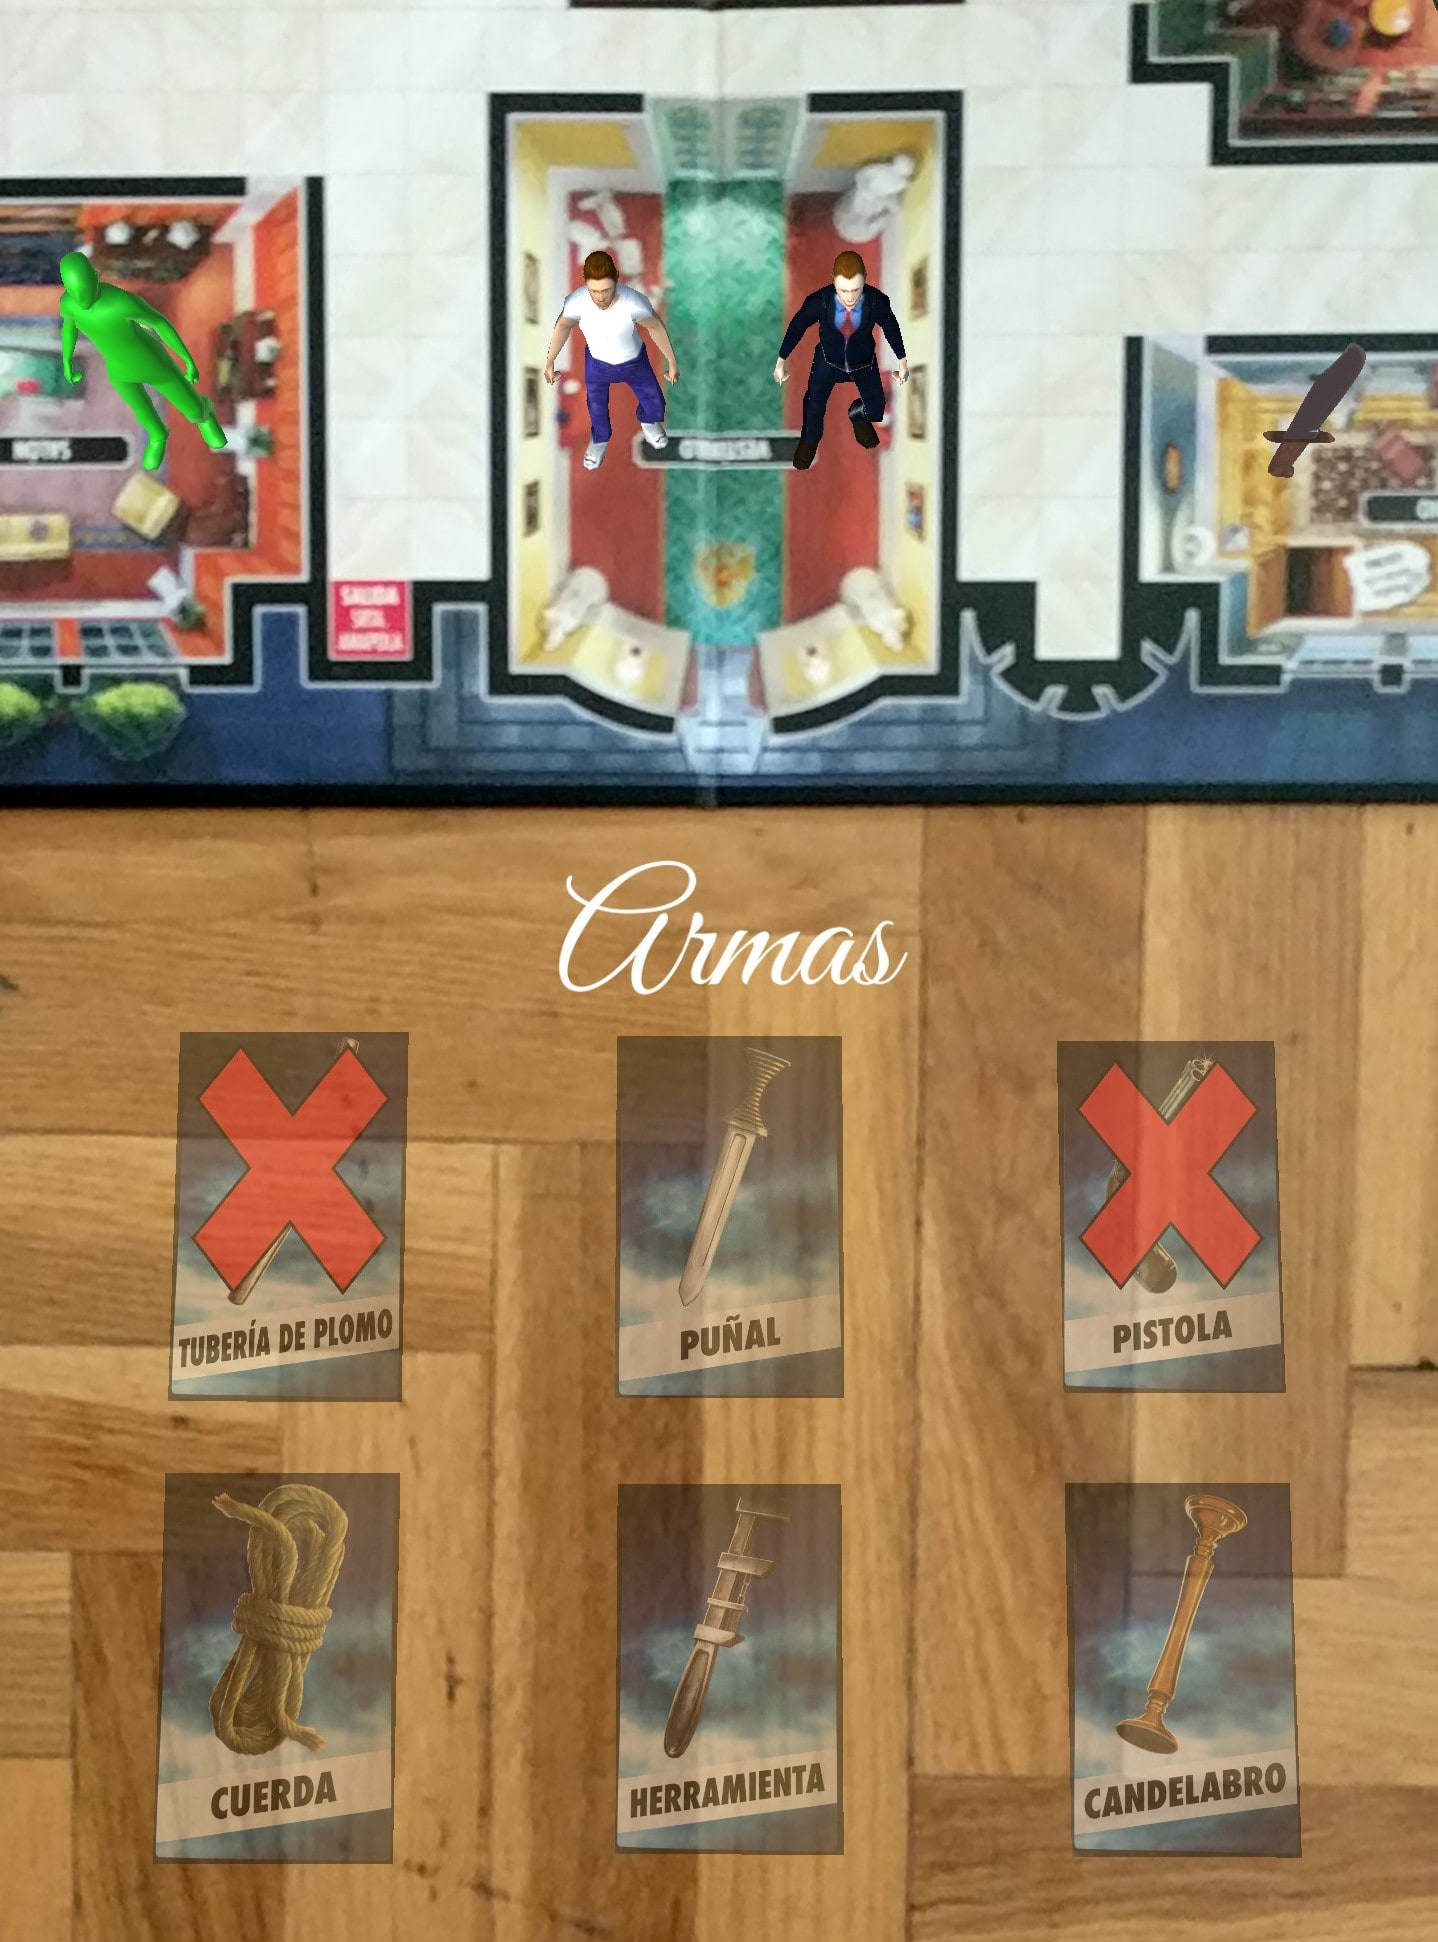
\includegraphics[scale=0.1]{notes-3}
  \caption{Imagen que muestra las cartas de armas tachadas y sin tachar.}
  \label{figura-notas-2}
\end{figure}

\newpage

En la figura \ref{figura-acus-1} se pueden observar los elementos que se muestran sobre las cartas escaneadas para una acusación.

\begin{figure}[h]
  \centering
  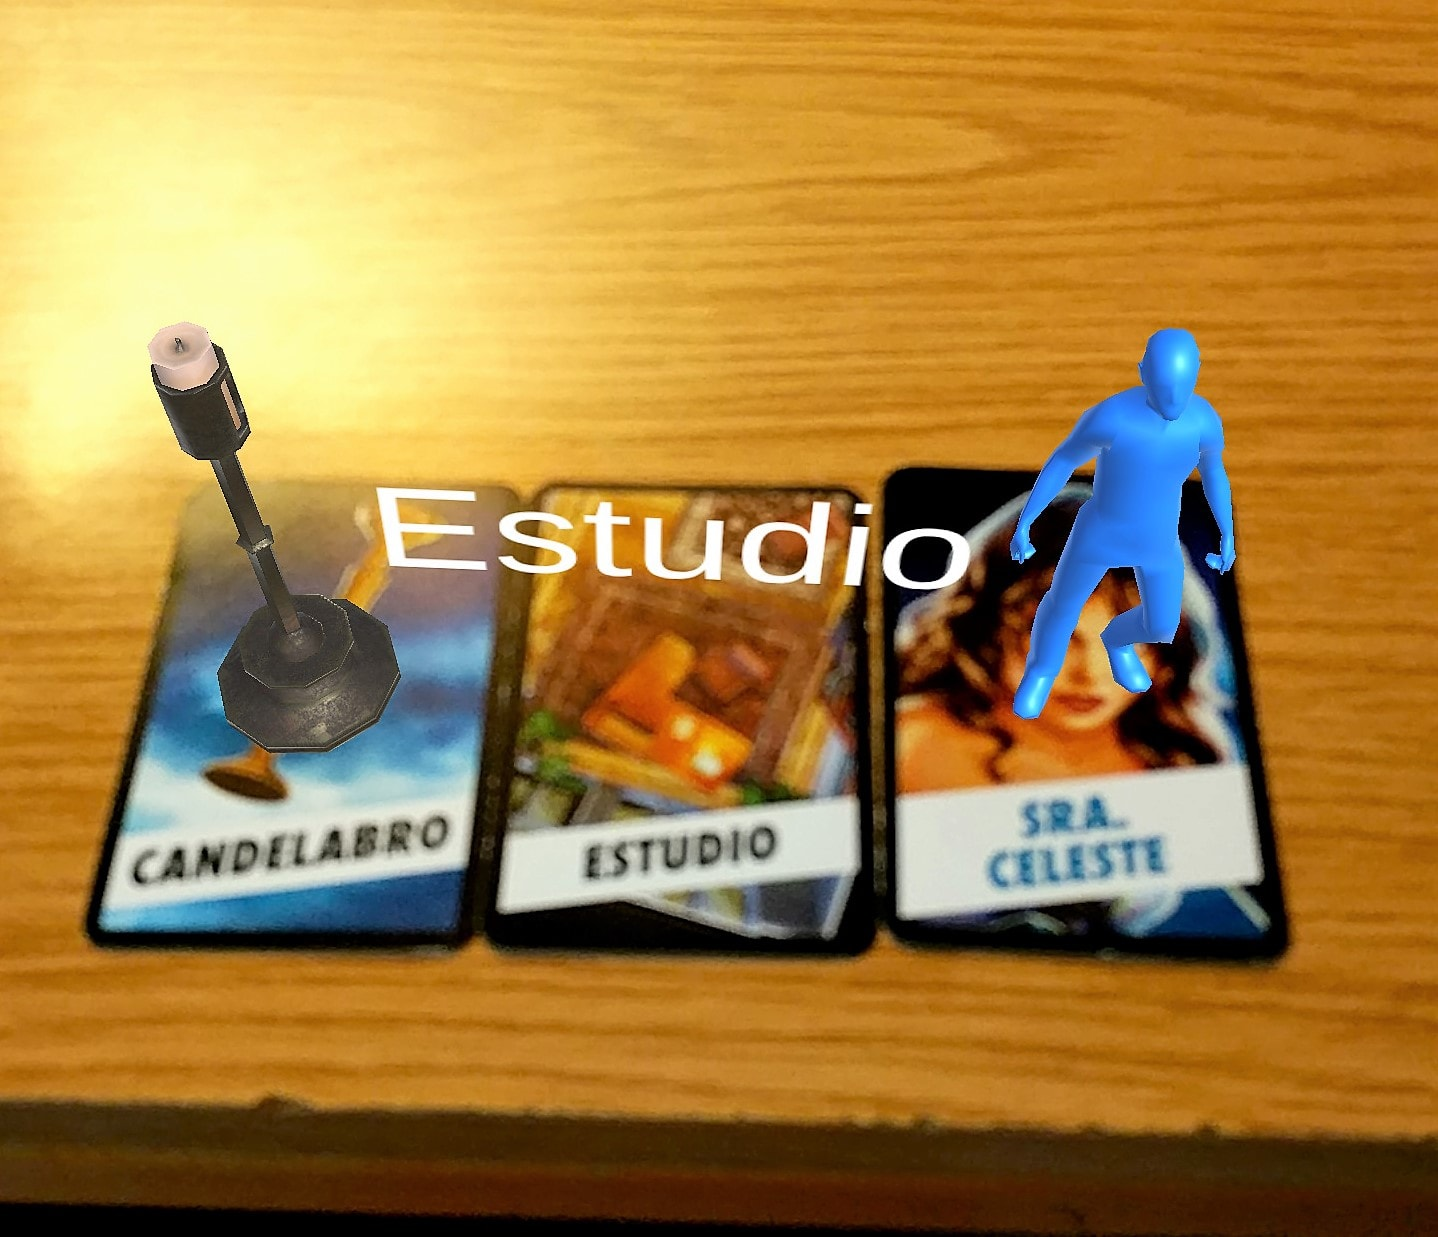
\includegraphics[scale=0.15]{acus-2}
  \caption{Imagen que muestra los elementos 3D posicionados sobre las cartas físicas.}
  \label{figura-acus-1}
\end{figure}

En la figura \ref{figura-fin-1} se puede observar la pantalla de finalización de partida a la que se llega una vez se realiza una acusación correcta.

\begin{figure}[h]
  \centering
  
\includegraphics[scale=0.07]{fin-1}
  \caption{Imagen que muestra la pantalla de finalización de partida.}
  \label{figura-fin-1}
\end{figure}

\subsection{Quinta iteración}
En esta iteración se han llevado a cabo las historias de usuario \ref{tabla-hu5} y \ref{tabla-hu6}.\\

Se ha desarrollado la funcionalidad de tirar los dados, de manera que al pulsar el botón "Lanzar dado", este se lanza, y una vez el dado para se muestran el resultado de lanzar el dado y las habitaciones disponibles para desplazarse en función de dicho resultado, el usuario tendrá que pulsar una de estas habitaciones para que el personaje se desplace a la habitación deseada, el resultado se muestre en la \textbf{Entrega 3}.\\

\subsection{Sexta iteración}
En esta iteración se han llevado a cabo las historias de usuario \ref{tabla-hu7} y \ref{tabla-hu8}.\\

Se ha desarrollado la funcionalidad de realizar una anotación, de manera que al pulsar el botón "Notas", se muestran las cartas de personajes, armas y habitaciones, y dichas cartas pueden ser pulsadas de forma que al pulsar se tacha dicha imagen para indicar que sabemos que ese no es el posible asesino, por ejemplo, y si se vuelve a pulsar una carta tachada, esta se desmarca, el resultado se muestre en la \textbf{Entrega 3}.\\

\subsection{Séptima iteración}
En esta iteración se han llevado a cabo las historias de usuario \ref{tabla-hu9} y \ref{tabla-hu10}.\\

Se ha desarrollado la funcionalidad de realizar una acusación, de manera que al escanear una carta mostrará un modelo 3D asociado a dicha carta, y al escanear tres cartas, un personaje, un arma y una habitación, se realizará la acusación comprobando si la combinación realizada es la correcta, el resultado se muestre en la \textbf{Entrega 3}.\\

También se ha desarrollado la pantalla de finalización de partida, de forma que si uno de los jugadores escanea la acusación correcta, se dirigirá a esta pantalla donde se indica el ganador y la finalización de partida, el resultado se muestra en la \textbf{Entrega 3}.\\

Por último, se realizaron pruebas con usuarios, poniéndoles en situación se les indicaba la tarea que tenían que hacer, y se fueron apuntando los problemas que estos tenían, detectando así elementos que mejorar en las funcionalidades realizadas en esta entrega. Los resultados de estas pruebas de usabilidad se encuentran en las Tablas \ref{tabla-entrega-3-usuario1}, \ref{tabla-entrega-3-usuario2} y \ref{tabla-entrega-3-usuario3}.


\subsection{Conclusiones}
Tras la realización de esta entrega se concluye que el proyecto avanza de forma favorable, todas las tareas se han llevado a cabo dentro de plazo y no han surgido grandes problemas.\\

Por otro lado, en las pruebas de usabilidad se comprueba que a pesar de desenvolverse de forma favorable en el juego, encuentran algunas dificultades. Estas dificultades son menores, pero pueden suponer una mejora considerable en cuanto a la usabilidad por parte de los usuarios, por tanto, se toman en cuenta y ser realizan los cambios correspondientes en el juego para solucionar dichas dificultades. Dichas dificultades se pueden encontrar en las tablas indicadas en la \textbf{Séptima iteración}.

\section{Entrega 4}
En esta entrega se ha completado la funcionalidad de pasar de turno, de forma que no solo se permitirá cambiar el turno pulsando un botón, si no que se ha creado toda la estructura necesaria para soportar dos jugadores en el juego con información diferente para cada uno de estos. Por otro lado también se ha desarrollado el sistema de pistas, que en función de la habitación en la que se encuentre el jugador actual se le darán pistas diferentes.\\

En la Figura \ref{figura-turn-1} se pueden observar los elementos que se muestran tras pulsar el botón de cambiar de turno, de forma que todos los elementos del tablero desaparecen y solo se muestra la interfaz de cambio de turno.

\begin{figure}[h]
  \centering
  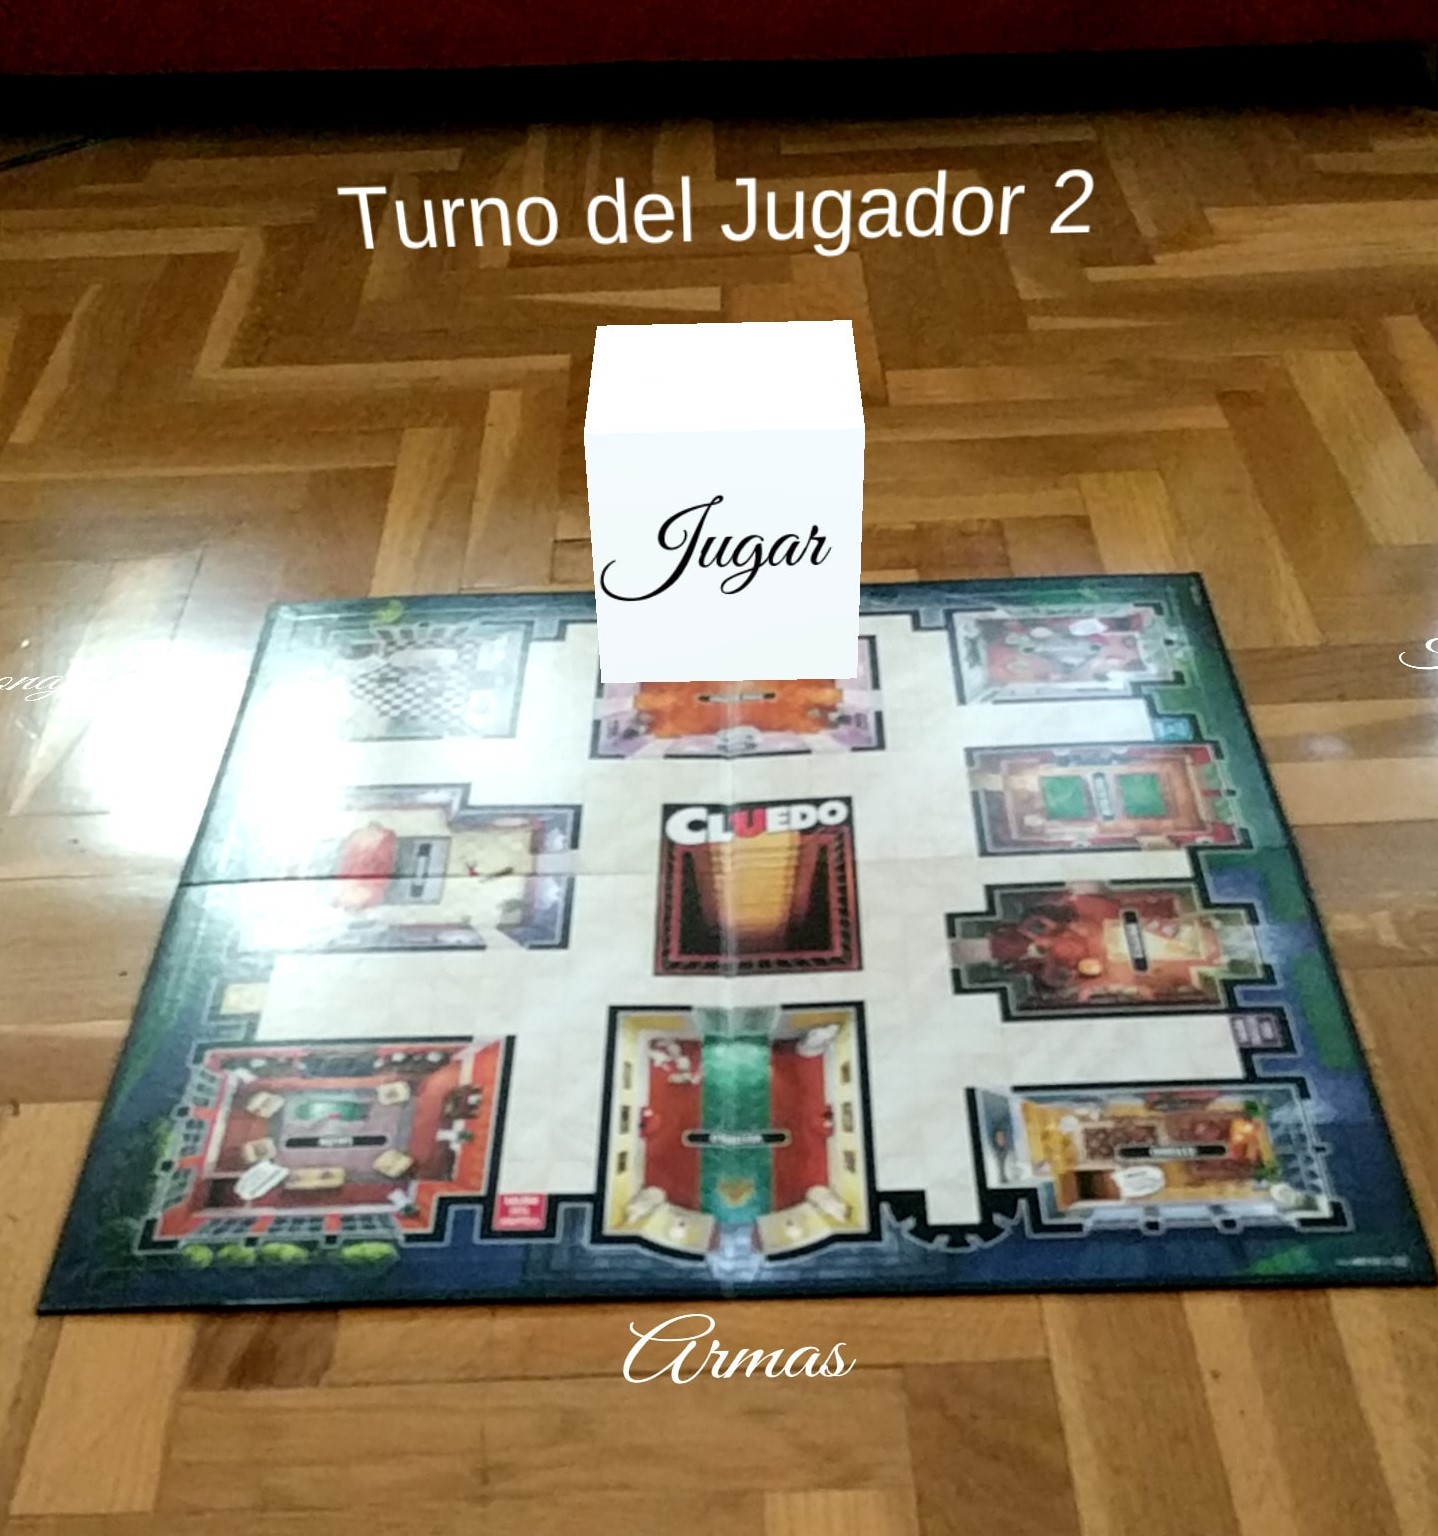
\includegraphics[scale=0.2]{turn-1}
  \caption{Imagen que muestra la interfaz de cambio de turno.}
  \label{figura-turn-1}
\end{figure}

\newpage

En la Figura \ref{figura-pista-1} se puede observar la interfaz de la pista recibida, con la pista y un botón para salir de dicha interfaz.

\begin{figure}[h]
  \centering
  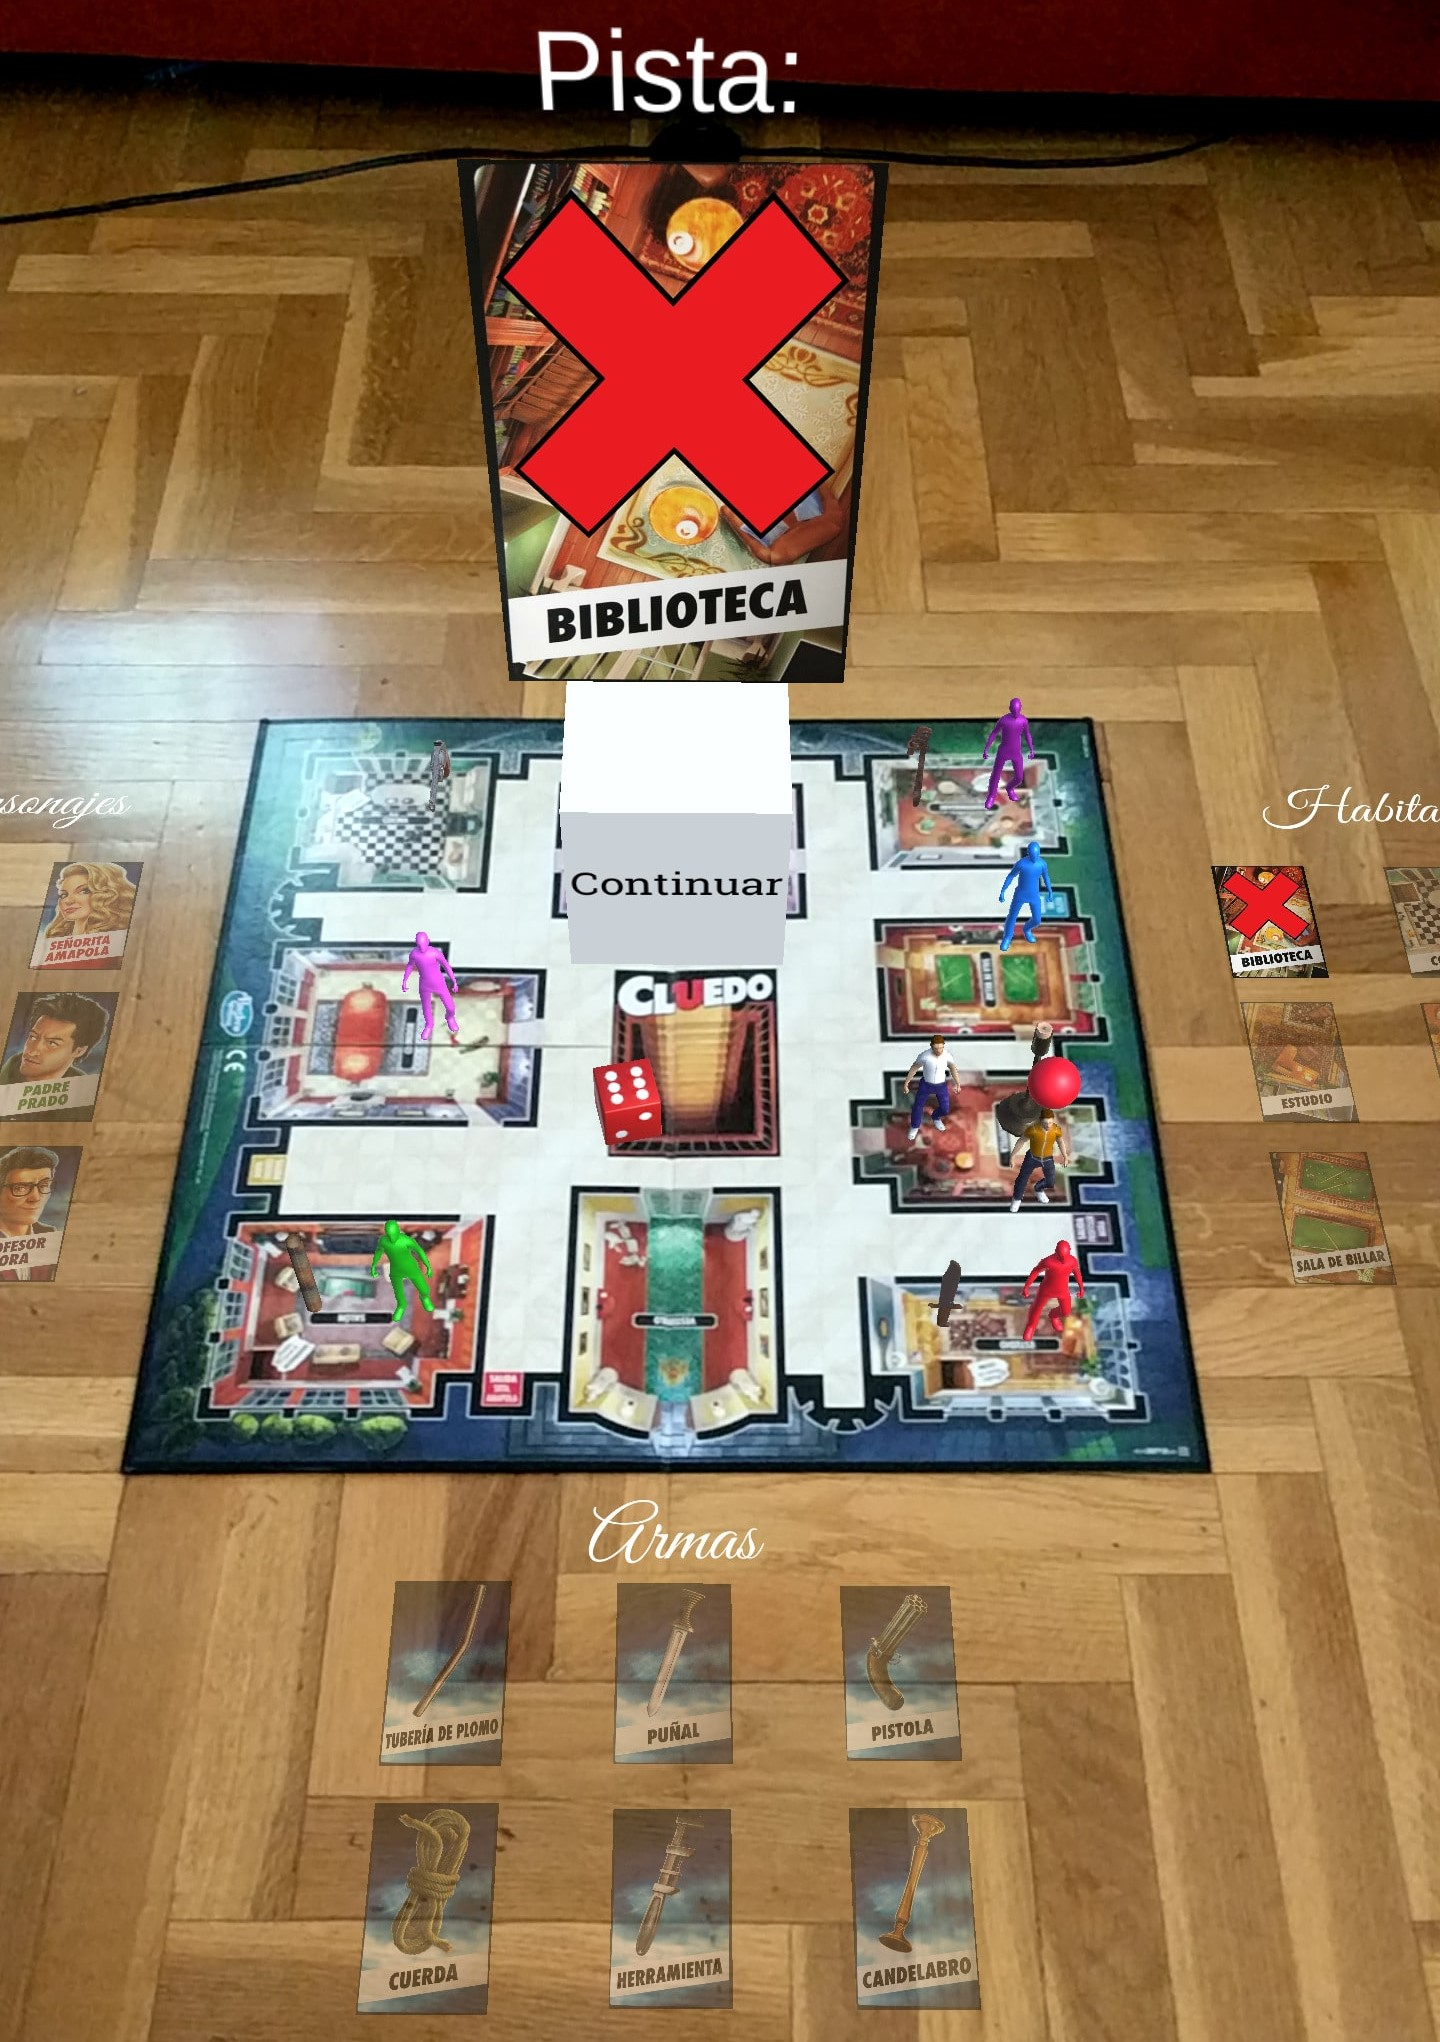
\includegraphics[scale=0.21]{pista-1}
  \caption{Imagen que muestra la carta de la pista y el botón para salir de dicha interfaz.}
  \label{figura-pista-1}
\end{figure}


\subsection{Octava iteración}
En esta iteración se ha llevado a cabo la historia de usuario \ref{tabla-hu11}.\\

En rasgos mas generales, en esta iteración se ha llevado a cabo el sistema de cambio de turno, que no solo implica la interfaz, si no también la modificación de la lógica del juego para que sea capaz de soportar mas de un usuario. Este cambio de turno implica información como las notas que es privada para cada usuario, por lo que se ha incluido una interfaz de cambio de turno en la que todos los elementos desaparecen para que una vez el usuario pasa de turno el siguiente pueda entrar en la pantalla de juego sin que se haya visto su información.\\

Como se puede observar en la Figura \ref{figura-code-multiuser}, para gestionar, por ejemplo, las notas de cada jugador se comprueba la variable turno, y en función del turno actual se comprueba las variables del jugador, por ejemplo, si tiene las notas activas pues se activaran dichos elementos 3D, si no las tienen activas pues no. Posteriormente se recorre un vector contenido en por un objeto ``Player" que se corresponde al jugador actual en función del turno, este indica que cartas el jugador ha marcado o desmarcado y cuales ha recibido como pista, y cada una de estas se muestra de una forma distinta, por ejemplo, si se ha recibido como una pista se muestra a pleno color y tachada. De esta forma a través de los mismos modelos 3D y en función de la información que se almacena en cada objeto ``Player" y en la variable turno entre otras, se puede establecer como se deben mostrar dichos elementos 3D en función del jugador que esta jugando en cada momento, permitiendo así un sistema multijugador sencillo de escalar.

\begin{figure}[h]
  \centering
  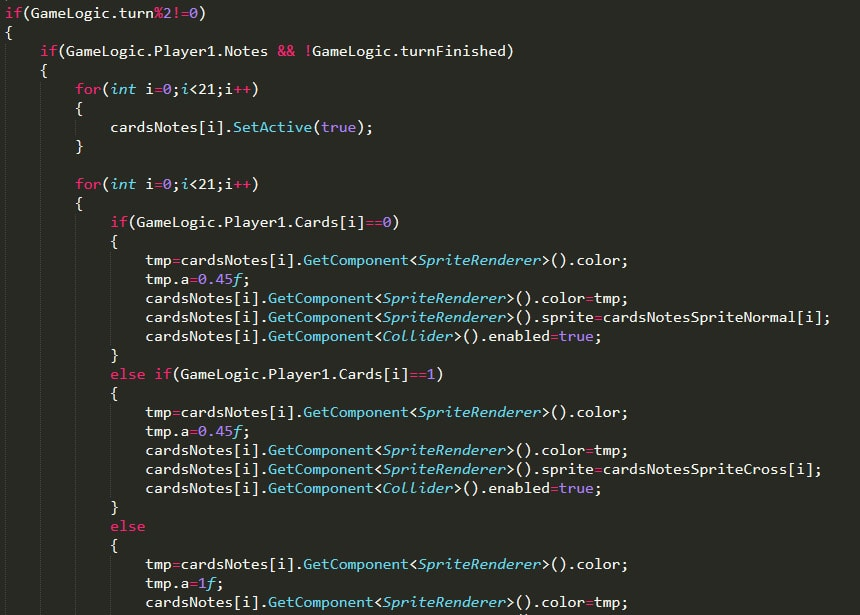
\includegraphics[scale=0.45]{code-multiuser}
  \caption{Imagen que muestra código de la gestión multiusuario.}
  \label{figura-code-multiuser}
\end{figure}

Por otro lado también se ha llevado a cabo el desarrollo del sistema de pistas, este se encarga de que cuando un usuario está en una habitación se le muestren pistas sobre los elementos que en esta se encuentran así como sobre la propia habitación, además de mostrarse esa pista, en la interfaz de notas la carta quedará marcada con una tonalidad diferente para que el usuario sea capaz de diferenciar dicha información como una pista, el resultado se muestra en la \textbf{Entrega 4}.\\

Por último, se realizaron pruebas con usuarios, poniéndoles en situación se les indicaba la tarea que tenían que hacer, y se fueron apuntando los problemas que estos tenían, detectando así elementos que mejorar en las funcionalidades realizadas en esta entrega. Los resultados de estas pruebas de usabilidad se encuentran en las Tablas \ref{tabla-entrega-4-usuario1}, \ref{tabla-entrega-4-usuario2} y \ref{tabla-entrega-4-usuario3}.


\subsection{Conclusiones}
Tras la realización de esta entrega se concluye que el proyecto ha avanzado de forma correcta y dentro de los plazos estimados, todas las tareas se han llevado a cabo a tiempo y no han surgido grandes problemas.\\

Por otro lado, en las pruebas de usabilidad se comprueba que los usuarios se desenvuelven con perfecta normalidad en el juego, sin encontrar ninguna dificultad en los cambios de turnos o al recibir pistas, por lo que se concluye que se han desarrollado dichas funcionalidades de forma exitosa.
